% Created 2025-06-08 Sun 17:13
% Intended LaTeX compiler: xelatex
\documentclass[11pt]{article}
\usepackage{capt-of}
\usepackage{hyperref}
% wrong resolution of image
% https://tex.stackexchange.com/questions/21627/image-from-includegraphics-showing-in-wrong-image-size?rq=1

%%%%%%%%%%%%%%%%%%%%%%%%%%%%%%%%%%%%%%
%% TIPS                                 %%
%%%%%%%%%%%%%%%%%%%%%%%%%%%%%%%%%%%%%%
% \substack{a\\b} for multiple lines text
% \usepackage{expl3}
% \expandafter\def\csname ver@l3regex.sty\endcsname{}
% \usepackage{pkgloader}
\usepackage[utf8]{inputenc}

% nfss error
% \usepackage[B1,T1]{fontenc}
\usepackage{fontspec}

% \usepackage[Emoticons]{ucharclasses}
\newfontfamily\DejaSans{DejaVu Sans}
% \setDefaultTransitions{\DejaSans}{}

% pdfplots will load xolor automatically without option
\usepackage[dvipsnames]{xcolor}

%                                                             ┳┳┓   ┓
%                                                             ┃┃┃┏┓╋┣┓
%                                                             ┛ ┗┗┻┗┛┗
% \usepackage{amsmath} mathtools loads the amsmath
\usepackage{amsmath}
\usepackage{mathtools}

\usepackage{amsthm}
\usepackage{amsbsy}

%\usepackage{commath}

\usepackage{amssymb}

\usepackage{mathrsfs}
%\usepackage{mathabx}
\usepackage{stmaryrd}
\usepackage{empheq}

\usepackage{scalerel}
\usepackage{stackengine}
\usepackage{stackrel}



\usepackage{nicematrix}
\usepackage{tensor}
\usepackage{blkarray}
\usepackage{siunitx}
\usepackage[f]{esvect}

% centering \not on a letter
\usepackage{slashed}
\usepackage[makeroom]{cancel}

%\usepackage{merriweather}
\usepackage{unicode-math}
\setmainfont{TeX Gyre Pagella}
% \setmathfont{STIX}
%\setmathfont{texgyrepagella-math.otf}
%\setmathfont{Libertinus Math}
\setmathfont{Latin Modern Math}

 % \setmathfont[range={\smwhtdiamond,\enclosediamond,\varlrtriangle}]{Latin Modern Math}
\setmathfont[range={\rightrightarrows,\twoheadrightarrow,\leftrightsquigarrow,\triangledown,\vartriangle,\precneq,\succneq,\prec,\succ,\preceq,\succeq,\tieconcat}]{XITS Math}
 \setmathfont[range={\int,\setminus}]{Libertinus Math}
 % \setmathfont[range={\mathalpha}]{TeX Gyre Pagella Math}
%\setmathfont[range={\mitA,\mitB,\mitC,\mitD,\mitE,\mitF,\mitG,\mitH,\mitI,\mitJ,\mitK,\mitL,\mitM,\mitN,\mitO,\mitP,\mitQ,\mitR,\mitS,\mitT,\mitU,\mitV,\mitW,\mitX,\mitY,\mitZ,\mita,\mitb,\mitc,\mitd,\mite,\mitf,\mitg,\miti,\mitj,\mitk,\mitl,\mitm,\mitn,\mito,\mitp,\mitq,\mitr,\mits,\mitt,\mitu,\mitv,\mitw,\mitx,\mity,\mitz}]{TeX Gyre Pagella Math}
% unicode is not good at this!
%\let\nmodels\nvDash

 \usepackage{wasysym}

 % for wide hat
 \DeclareSymbolFont{yhlargesymbols}{OMX}{yhex}{m}{n} \DeclareMathAccent{\what}{\mathord}{yhlargesymbols}{"62}

%                                                               ┏┳┓•┓
%                                                                ┃ ┓┃┏┓
%                                                                ┻ ┗┛┗┗

\usepackage{pgfplots}
\pgfplotsset{compat=1.18}
\usepackage{tikz}
\usepackage{tikz-cd}
\tikzcdset{scale cd/.style={every label/.append style={scale=#1},
    cells={nodes={scale=#1}}}}
% TODO: discard qtree and use forest
% \usepackage{tikz-qtree}
\usepackage{forest}

\usetikzlibrary{arrows,positioning,calc,fadings,decorations,matrix,decorations,shapes.misc}
%setting from geogebra
\definecolor{ccqqqq}{rgb}{0.8,0,0}

%                                                          ┳┳┓•    ┓┓
%                                                          ┃┃┃┓┏┏┏┓┃┃┏┓┏┓┏┓┏┓┓┏┏
%                                                          ┛ ┗┗┛┗┗ ┗┗┗┻┛┗┗ ┗┛┗┻┛
%\usepackage{twemojis}
\usepackage[most]{tcolorbox}
\usepackage{threeparttable}
\usepackage{tabularx}

\usepackage{enumitem}
\usepackage[indLines=false]{algpseudocodex}
\usepackage[]{algorithm2e}
% \SetKwComment{Comment}{/* }{ */}
% \algrenewcommand\algorithmicrequire{\textbf{Input:}}
% \algrenewcommand\algorithmicensure{\textbf{Output:}}
% wrong with preview
\usepackage{subcaption}
\usepackage{caption}
% {\aunclfamily\Huge}
\usepackage{auncial}

\usepackage{float}

\usepackage{fancyhdr}

\usepackage{ifthen}
\usepackage{xargs}

\definecolor{mintedbg}{rgb}{0.99,0.99,0.99}
\usepackage[cachedir=\detokenize{~/miscellaneous/trash}]{minted}
\setminted{breaklines,
  mathescape,
  bgcolor=mintedbg,
  fontsize=\footnotesize,
  frame=single,
  linenos}
\usemintedstyle{xcode}
\usepackage{tcolorbox}
\usepackage{etoolbox}



\usepackage{imakeidx}
\usepackage{hyperref}
\usepackage{soul}
\usepackage{framed}

% don't use this for preview
%\usepackage[margin=1.5in]{geometry}
% \usepackage{geometry}
% \geometry{legalpaper, landscape, margin=1in}
\usepackage[font=itshape]{quoting}

%\LoadPackagesNow
%\usepackage[xetex]{preview}
%%%%%%%%%%%%%%%%%%%%%%%%%%%%%%%%%%%%%%%
%% USEPACKAGES end                       %%
%%%%%%%%%%%%%%%%%%%%%%%%%%%%%%%%%%%%%%%

%%%%%%%%%%%%%%%%%%%%%%%%%%%%%%%%%%%%%%%
%% Algorithm environment
%%%%%%%%%%%%%%%%%%%%%%%%%%%%%%%%%%%%%%%
\SetKwIF{Recv}{}{}{upon receiving}{do}{}{}{}
\SetKwBlock{Init}{initially do}{}
\SetKwProg{Function}{Function}{:}{}

% https://github.com/chrmatt/algpseudocodex/issues/3
\algnewcommand\algorithmicswitch{\textbf{switch}}%
\algnewcommand\algorithmiccase{\textbf{case}}
\algnewcommand\algorithmicof{\textbf{of}}
\algnewcommand\algorithmicotherwise{\texttt{otherwise} $\Rightarrow$}

\makeatletter
\algdef{SE}[SWITCH]{Switch}{EndSwitch}[1]{\algpx@startIndent\algpx@startCodeCommand\algorithmicswitch\ #1\ \algorithmicdo}{\algpx@endIndent\algpx@startCodeCommand\algorithmicend\ \algorithmicswitch}%
\algdef{SE}[CASE]{Case}{EndCase}[1]{\algpx@startIndent\algpx@startCodeCommand\algorithmiccase\ #1}{\algpx@endIndent\algpx@startCodeCommand\algorithmicend\ \algorithmiccase}%
\algdef{SE}[CASEOF]{CaseOf}{EndCaseOf}[1]{\algpx@startIndent\algpx@startCodeCommand\algorithmiccase\ #1 \algorithmicof}{\algpx@endIndent\algpx@startCodeCommand\algorithmicend\ \algorithmiccase}
\algdef{SE}[OTHERWISE]{Otherwise}{EndOtherwise}[0]{\algpx@startIndent\algpx@startCodeCommand\algorithmicotherwise}{\algpx@endIndent\algpx@startCodeCommand\algorithmicend\ \algorithmicotherwise}
\ifbool{algpx@noEnd}{%
  \algtext*{EndSwitch}%
  \algtext*{EndCase}%
  \algtext*{EndCaseOf}
  \algtext*{EndOtherwise}
  %
  % end indent line after (not before), to get correct y position for multiline text in last command
  \apptocmd{\EndSwitch}{\algpx@endIndent}{}{}%
  \apptocmd{\EndCase}{\algpx@endIndent}{}{}%
  \apptocmd{\EndCaseOf}{\algpx@endIndent}{}{}
  \apptocmd{\EndOtherwise}{\algpx@endIndent}{}{}
}{}%

\pretocmd{\Switch}{\algpx@endCodeCommand}{}{}
\pretocmd{\Case}{\algpx@endCodeCommand}{}{}
\pretocmd{\CaseOf}{\algpx@endCodeCommand}{}{}
\pretocmd{\Otherwise}{\algpx@endCodeCommand}{}{}

% for end commands that may not be printed, tell endCodeCommand whether we are using noEnd
\ifbool{algpx@noEnd}{%
  \pretocmd{\EndSwitch}{\algpx@endCodeCommand[1]}{}{}%
  \pretocmd{\EndCase}{\algpx@endCodeCommand[1]}{}{}
  \pretocmd{\EndCaseOf}{\algpx@endCodeCommand[1]}{}{}%
  \pretocmd{\EndOtherwise}{\algpx@endCodeCommand[1]}{}{}
}{%
  \pretocmd{\EndSwitch}{\algpx@endCodeCommand[0]}{}{}%
  \pretocmd{\EndCase}{\algpx@endCodeCommand[0]}{}{}%
  \pretocmd{\EndCaseOf}{\algpx@endCodeCommand[0]}{}{}
  \pretocmd{\EndOtherwise}{\algpx@endCodeCommand[0]}{}{}
}%
\makeatother
% % For algpseudocode
% \algnewcommand\algorithmicswitch{\textbf{switch}}
% \algnewcommand\algorithmiccase{\textbf{case}}
% \algnewcommand\algorithmiccaseof{\textbf{case}}
% \algnewcommand\algorithmicof{\textbf{of}}
% % New "environments"
% \algdef{SE}[SWITCH]{Switch}{EndSwitch}[1]{\algorithmicswitch\ #1\ \algorithmicdo}{\algorithmicend\ \algorithmicswitch}%
% \algdef{SE}[CASE]{Case}{EndCase}[1]{\algorithmiccase\ #1}{\algorithmicend\ \algorithmiccase}%
% \algtext*{EndSwitch}%
% \algtext*{EndCase}
% \algdef{SE}[CASEOF]{CaseOf}{EndCaseOf}[1]{\algorithmiccaseof\ #1 \algorithmicof}{\algorithmicend\ \algorithmiccaseof}
% \algtext*{EndCaseOf}



%\pdfcompresslevel0

% quoting from
% https://tex.stackexchange.com/questions/391726/the-quotation-environment
\NewDocumentCommand{\bywhom}{m}{% the Bourbaki trick
  {\nobreak\hfill\penalty50\hskip1em\null\nobreak
   \hfill\mbox{\normalfont(#1)}%
   \parfillskip=0pt \finalhyphendemerits=0 \par}%
}

\NewDocumentEnvironment{pquotation}{m}
  {\begin{quoting}[
     indentfirst=true,
     leftmargin=\parindent,
     rightmargin=\parindent]\itshape}
  {\bywhom{#1}\end{quoting}}

\indexsetup{othercode=\small}
\makeindex[columns=2,options={-s /media/wu/file/stuuudy/notes/index_style.ist},intoc]
\makeatletter
\def\@idxitem{\par\hangindent 0pt}
\makeatother


% \newcounter{dummy} \numberwithin{dummy}{section}
\newtheorem{dummy}{dummy}[section]
\theoremstyle{definition}
\newtheorem{definition}[dummy]{Definition}
\theoremstyle{plain}
\newtheorem{corollary}[dummy]{Corollary}
\newtheorem{lemma}[dummy]{Lemma}
\newtheorem{proposition}[dummy]{Proposition}
\newtheorem{theorem}[dummy]{Theorem}
\newtheorem{notation}[dummy]{Notation}
\newtheorem{conjecture}[dummy]{Conjecture}
\newtheorem{fact}[dummy]{Fact}
\newtheorem{warning}[dummy]{Warning}
\theoremstyle{definition}
\newtheorem{examplle}{Example}[section]
\theoremstyle{remark}
\newtheorem*{remark}{Remark}
\newtheorem{exercise}{Exercise}[subsection]
\newtheorem{problem}{Problem}[subsection]
\newtheorem{observation}{Observation}[section]
\newenvironment{claim}[1]{\par\noindent\textbf{Claim:}\space#1}{}

\makeatletter
\DeclareFontFamily{U}{tipa}{}
\DeclareFontShape{U}{tipa}{m}{n}{<->tipa10}{}
\newcommand{\arc@char}{{\usefont{U}{tipa}{m}{n}\symbol{62}}}%

\newcommand{\arc}[1]{\mathpalette\arc@arc{#1}}

\newcommand{\arc@arc}[2]{%
  \sbox0{$\m@th#1#2$}%
  \vbox{
    \hbox{\resizebox{\wd0}{\height}{\arc@char}}
    \nointerlineskip
    \box0
  }%
}
\makeatother

\setcounter{MaxMatrixCols}{20}
%%%%%%% ABS
\DeclarePairedDelimiter\abss{\lvert}{\rvert}%
\DeclarePairedDelimiter\normm{\lVert}{\rVert}%

% Swap the definition of \abs* and \norm*, so that \abs
% and \norm resizes the size of the brackets, and the
% starred version does not.
\makeatletter
\let\oldabs\abss
%\def\abs{\@ifstar{\oldabs}{\oldabs*}}
\newcommand{\abs}{\@ifstar{\oldabs}{\oldabs*}}
\newcommand{\norm}[1]{\left\lVert#1\right\rVert}
%\let\oldnorm\normm
%\def\norm{\@ifstar{\oldnorm}{\oldnorm*}}
%\renewcommand{norm}{\@ifstar{\oldnorm}{\oldnorm*}}
\makeatother

% \stackMath
% \newcommand\what[1]{%
% \savestack{\tmpbox}{\stretchto{%
%   \scaleto{%
%     \scalerel*[\widthof{\ensuremath{#1}}]{\kern-.6pt\bigwedge\kern-.6pt}%
%     {\rule[-\textheight/2]{1ex}{\textheight}}%WIDTH-LIMITED BIG WEDGE
%   }{\textheight}%
% }{0.5ex}}%
% \stackon[1pt]{#1}{\tmpbox}%
% }

% \newcommand\what[1]{\ThisStyle{%
%     \setbox0=\hbox{$\SavedStyle#1$}%
%     \stackengine{-1.0\ht0+.5pt}{$\SavedStyle#1$}{%
%       \stretchto{\scaleto{\SavedStyle\mkern.15mu\char'136}{2.6\wd0}}{1.4\ht0}%
%     }{O}{c}{F}{T}{S}%
%   }
% }

% \newcommand\wtilde[1]{\ThisStyle{%
%     \setbox0=\hbox{$\SavedStyle#1$}%
%     \stackengine{-.1\LMpt}{$\SavedStyle#1$}{%
%       \stretchto{\scaleto{\SavedStyle\mkern.2mu\AC}{.5150\wd0}}{.6\ht0}%
%     }{O}{c}{F}{T}{S}%
%   }
% }

% \newcommand\wbar[1]{\ThisStyle{%
%     \setbox0=\hbox{$\SavedStyle#1$}%
%     \stackengine{.5pt+\LMpt}{$\SavedStyle#1$}{%
%       \rule{\wd0}{\dimexpr.3\LMpt+.3pt}%
%     }{O}{c}{F}{T}{S}%
%   }
% }

\newcommand{\bl}[1] {\boldsymbol{#1}}
\newcommand{\Wt}[1] {\stackrel{\sim}{\smash{#1}\rule{0pt}{1.1ex}}}
\newcommand{\wt}[1] {\widetilde{#1}}
\newcommand{\tf}[1] {\textbf{#1}}

\newcommand{\wu}[1]{{\color{red} #1}}

%For boxed texts in align, use Aboxed{}
%otherwise use boxed{}

\DeclareMathSymbol{\widehatsym}{\mathord}{largesymbols}{"62}
\newcommand\lowerwidehatsym{%
  \text{\smash{\raisebox{-1.3ex}{%
    $\widehatsym$}}}}
\newcommand\fixwidehat[1]{%
  \mathchoice
    {\accentset{\displaystyle\lowerwidehatsym}{#1}}
    {\accentset{\textstyle\lowerwidehatsym}{#1}}
    {\accentset{\scriptstyle\lowerwidehatsym}{#1}}
    {\accentset{\scriptscriptstyle\lowerwidehatsym}{#1}}
  }


\newcommand{\cupdot}{\mathbin{\dot{\cup}}}
\newcommand{\bigcupdot}{\mathop{\dot{\bigcup}}}

\usepackage{graphicx}

\usepackage[toc,page]{appendix}

% text on arrow for xRightarrow
\makeatletter
%\newcommand{\xRightarrow}[2][]{\ext@arrow 0359\Rightarrowfill@{#1}{#2}}
\makeatother

% Arbitrary long arrow
\newcommand{\Rarrow}[1]{%
\parbox{#1}{\tikz{\draw[->](0,0)--(#1,0);}}
}

\newcommand{\LRarrow}[1]{%
\parbox{#1}{\tikz{\draw[<->](0,0)--(#1,0);}}
}


\makeatletter
\providecommand*{\rmodels}{%
  \mathrel{%
    \mathpalette\@rmodels\models
  }%
}
\newcommand*{\@rmodels}[2]{%
  \reflectbox{$\m@th#1#2$}%
}
\makeatother

% Roman numerals
\makeatletter
\newcommand*{\rom}[1]{\expandafter\@slowromancap\romannumeral #1@}
\makeatother
% \\def \\b\([a-zA-Z]\) {\\boldsymbol{[a-zA-z]}}
% \\DeclareMathOperator{\\b\1}{\\textbf{\1}}

\DeclareMathOperator*{\argmin}{arg\,min}
\DeclareMathOperator*{\argmax}{arg\,max}

\DeclareMathOperator{\bone}{\textbf{1}}
\DeclareMathOperator{\bx}{\textbf{x}}
\DeclareMathOperator{\bz}{\textbf{z}}
\DeclareMathOperator{\bff}{\textbf{f}}
\DeclareMathOperator{\ba}{\textbf{a}}
\DeclareMathOperator{\bk}{\textbf{k}}
\DeclareMathOperator{\bs}{\textbf{s}}
\DeclareMathOperator{\bh}{\textbf{h}}
\DeclareMathOperator{\bc}{\textbf{c}}
\DeclareMathOperator{\br}{\textbf{r}}
\DeclareMathOperator{\bi}{\textbf{i}}
\DeclareMathOperator{\bj}{\textbf{j}}
\DeclareMathOperator{\bn}{\textbf{n}}
\DeclareMathOperator{\be}{\textbf{e}}
\DeclareMathOperator{\bo}{\textbf{o}}
\DeclareMathOperator{\bU}{\textbf{U}}
\DeclareMathOperator{\bL}{\textbf{L}}
\DeclareMathOperator{\bV}{\textbf{V}}
\def \bzero {\mathbf{0}}
\def \bbone {\mathbb{1}}
\def \btwo {\mathbf{2}}
\DeclareMathOperator{\bv}{\textbf{v}}
\DeclareMathOperator{\bp}{\textbf{p}}
\DeclareMathOperator{\bI}{\textbf{I}}
\def \dbI {\dot{\bI}}
\DeclareMathOperator{\bM}{\textbf{M}}
\DeclareMathOperator{\bN}{\textbf{N}}
\DeclareMathOperator{\bK}{\textbf{K}}
\DeclareMathOperator{\bt}{\textbf{t}}
\DeclareMathOperator{\bb}{\textbf{b}}
\DeclareMathOperator{\bA}{\textbf{A}}
\DeclareMathOperator{\bX}{\textbf{X}}
\DeclareMathOperator{\bu}{\textbf{u}}
\DeclareMathOperator{\bS}{\textbf{S}}
\DeclareMathOperator{\bZ}{\textbf{Z}}
\DeclareMathOperator{\bJ}{\textbf{J}}
\DeclareMathOperator{\by}{\textbf{y}}
\DeclareMathOperator{\bw}{\textbf{w}}
\DeclareMathOperator{\bT}{\textbf{T}}
\DeclareMathOperator{\bF}{\textbf{F}}
\DeclareMathOperator{\bmm}{\textbf{m}}
\DeclareMathOperator{\bW}{\textbf{W}}
\DeclareMathOperator{\bR}{\textbf{R}}
\DeclareMathOperator{\bC}{\textbf{C}}
\DeclareMathOperator{\bD}{\textbf{D}}
\DeclareMathOperator{\bE}{\textbf{E}}
\DeclareMathOperator{\bQ}{\textbf{Q}}
\DeclareMathOperator{\bP}{\textbf{P}}
\DeclareMathOperator{\bY}{\textbf{Y}}
\DeclareMathOperator{\bH}{\textbf{H}}
\DeclareMathOperator{\bB}{\textbf{B}}
\DeclareMathOperator{\bG}{\textbf{G}}
\def \blambda {\symbf{\lambda}}
\def \boldeta {\symbf{\eta}}
\def \balpha {\symbf{\alpha}}
\def \btau {\symbf{\tau}}
\def \bbeta {\symbf{\beta}}
\def \bgamma {\symbf{\gamma}}
\def \bxi {\symbf{\xi}}
\def \bLambda {\symbf{\Lambda}}
\def \bGamma {\symbf{\Gamma}}

\newcommand{\bto}{{\boldsymbol{\to}}}
\newcommand{\Ra}{\Rightarrow}
\newcommand{\xrsa}[1]{\overset{#1}{\rightsquigarrow}}
\newcommand{\xlsa}[1]{\overset{#1}{\leftsquigarrow}}
\newcommand\und[1]{\underline{#1}}
\newcommand\ove[1]{\overline{#1}}
%\def \concat {\verb|^|}
\def \bPhi {\mbfPhi}
\def \btheta {\mbftheta}
\def \bTheta {\mbfTheta}
\def \bmu {\mbfmu}
\def \bphi {\mbfphi}
\def \bSigma {\mbfSigma}
\def \la {\langle}
\def \ra {\rangle}

\def \caln {\mathcal{N}}
\def \dissum {\displaystyle\Sigma}
\def \dispro {\displaystyle\prod}

\def \caret {\verb!^!}

\def \A {\mathbb{A}}
\def \B {\mathbb{B}}
\def \C {\mathbb{C}}
\def \D {\mathbb{D}}
\def \E {\mathbb{E}}
\def \F {\mathbb{F}}
\def \G {\mathbb{G}}
\def \H {\mathbb{H}}
\def \I {\mathbb{I}}
\def \J {\mathbb{J}}
\def \K {\mathbb{K}}
\def \L {\mathbb{L}}
\def \M {\mathbb{M}}
\def \N {\mathbb{N}}
\def \O {\mathbb{O}}
\def \P {\mathbb{P}}
\def \Q {\mathbb{Q}}
\def \R {\mathbb{R}}
\def \S {\mathbb{S}}
\def \T {\mathbb{T}}
\def \U {\mathbb{U}}
\def \V {\mathbb{V}}
\def \W {\mathbb{W}}
\def \X {\mathbb{X}}
\def \Y {\mathbb{Y}}
\def \Z {\mathbb{Z}}

\def \cala {\mathcal{A}}
\def \cale {\mathcal{E}}
\def \calb {\mathcal{B}}
\def \calq {\mathcal{Q}}
\def \calp {\mathcal{P}}
\def \cals {\mathcal{S}}
\def \calx {\mathcal{X}}
\def \caly {\mathcal{Y}}
\def \calg {\mathcal{G}}
\def \cald {\mathcal{D}}
\def \caln {\mathcal{N}}
\def \calr {\mathcal{R}}
\def \calt {\mathcal{T}}
\def \calm {\mathcal{M}}
\def \calw {\mathcal{W}}
\def \calc {\mathcal{C}}
\def \calv {\mathcal{V}}
\def \calf {\mathcal{F}}
\def \calk {\mathcal{K}}
\def \call {\mathcal{L}}
\def \calu {\mathcal{U}}
\def \calo {\mathcal{O}}
\def \calh {\mathcal{H}}
\def \cali {\mathcal{I}}
\def \calj {\mathcal{J}}

\def \bcup {\bigcup}

% set theory

\def \zfcc {\textbf{ZFC}^-}
\def \BGC {\textbf{BGC}}
\def \BG {\textbf{BG}}
\def \ac  {\textbf{AC}}
\def \gl  {\textbf{L }}
\def \gll {\textbf{L}}
\newcommand{\zfm}{$\textbf{ZF}^-$}

\def \ZFm {\text{ZF}^-}
\def \ZFCm {\text{ZFC}^-}
\DeclareMathOperator{\WF}{WF}
\DeclareMathOperator{\On}{On}
\def \on {\textbf{On }}
\def \cm {\textbf{M }}
\def \cn {\textbf{N }}
\def \cv {\textbf{V }}
\def \zc {\textbf{ZC }}
\def \zcm {\textbf{ZC}}
\def \zff {\textbf{ZF}}
\def \wfm {\textbf{WF}}
\def \onm {\textbf{On}}
\def \cmm {\textbf{M}}
\def \cnm {\textbf{N}}
\def \cvm {\textbf{V}}

\renewcommand{\restriction}{\mathord{\upharpoonright}}
%% another restriction
\newcommand\restr[2]{{% we make the whole thing an ordinary symbol
  \left.\kern-\nulldelimiterspace % automatically resize the bar with \right
  #1 % the function
  \vphantom{\big|} % pretend it's a little taller at normal size
  \right|_{#2} % this is the delimiter
  }}

\def \pred {\text{pred}}

\def \rank {\text{rank}}
\def \Con {\text{Con}}
\def \deff {\text{Def}}


\def \uin {\underline{\in}}
\def \oin {\overline{\in}}
\def \uR {\underline{R}}
\def \oR {\overline{R}}
\def \uP {\underline{P}}
\def \oP {\overline{P}}

\def \dsum {\displaystyle\sum}

\def \Ra {\Rightarrow}

\def \e {\enspace}

\def \sgn {\operatorname{sgn}}
\def \gen {\operatorname{gen}}
\def \Hom {\operatorname{Hom}}
\def \hom {\operatorname{hom}}
\def \Sub {\operatorname{Sub}}

\def \supp {\operatorname{supp}}

\def \epiarrow {\twoheadarrow}
\def \monoarrow {\rightarrowtail}
\def \rrarrow {\rightrightarrows}

% \def \minus {\text{-}}
% \newcommand{\minus}{\scalebox{0.75}[1.0]{$-$}}
% \DeclareUnicodeCharacter{002D}{\minus}


\def \tril {\triangleleft}

\def \ISigma {\text{I}\Sigma}
\def \IDelta {\text{I}\Delta}
\def \IPi {\text{I}\Pi}
\def \ACF {\textsf{ACF}}
\def \pCF {\textit{p}\text{CF}}
\def \ACVF {\textsf{ACVF}}
\def \HLR {\textsf{HLR}}
\def \OAG {\textsf{OAG}}
\def \RCF {\textsf{RCF}}
\DeclareMathOperator{\GL}{GL}
\DeclareMathOperator{\PGL}{PGL}
\DeclareMathOperator{\SL}{SL}
\DeclareMathOperator{\Inv}{Inv}
\DeclareMathOperator{\res}{res}
\DeclareMathOperator{\Sym}{Sym}
%\DeclareMathOperator{\char}{char}
\def \equal {=}

\def \degree {\text{degree}}
\def \app {\text{App}}
\def \FV {\text{FV}}
\def \conv {\text{conv}}
\def \cont {\text{cont}}
\DeclareMathOperator{\cl}{\text{cl}}
\DeclareMathOperator{\trcl}{\text{trcl}}
\DeclareMathOperator{\sg}{sg}
\DeclareMathOperator{\trdeg}{trdeg}
\def \Ord {\text{Ord}}

\DeclareMathOperator{\cf}{cf}
\DeclareMathOperator{\zfc}{ZFC}

%\DeclareMathOperator{\Th}{Th}
%\def \th {\text{Th}}
% \newcommand{\th}{\text{Th}}
\DeclareMathOperator{\type}{type}
\DeclareMathOperator{\zf}{\textbf{ZF}}
\def \fa {\mathfrak{a}}
\def \fb {\mathfrak{b}}
\def \fc {\mathfrak{c}}
\def \fd {\mathfrak{d}}
\def \fe {\mathfrak{e}}
\def \ff {\mathfrak{f}}
\def \fg {\mathfrak{g}}
\def \fh {\mathfrak{h}}
%\def \fi {\mathfrak{i}}
\def \fj {\mathfrak{j}}
\def \fk {\mathfrak{k}}
\def \fl {\mathfrak{l}}
\def \fm {\mathfrak{m}}
\def \fn {\mathfrak{n}}
\def \fo {\mathfrak{o}}
\def \fp {\mathfrak{p}}
\def \fq {\mathfrak{q}}
\def \fr {\mathfrak{r}}
\def \fs {\mathfrak{s}}
\def \ft {\mathfrak{t}}
\def \fu {\mathfrak{u}}
\def \fv {\mathfrak{v}}
\def \fw {\mathfrak{w}}
\def \fx {\mathfrak{x}}
\def \fy {\mathfrak{y}}
\def \fz {\mathfrak{z}}
\def \fA {\mathfrak{A}}
\def \fB {\mathfrak{B}}
\def \fC {\mathfrak{C}}
\def \fD {\mathfrak{D}}
\def \fE {\mathfrak{E}}
\def \fF {\mathfrak{F}}
\def \fG {\mathfrak{G}}
\def \fH {\mathfrak{H}}
\def \fI {\mathfrak{I}}
\def \fJ {\mathfrak{J}}
\def \fK {\mathfrak{K}}
\def \fL {\mathfrak{L}}
\def \fM {\mathfrak{M}}
\def \fN {\mathfrak{N}}
\def \fO {\mathfrak{O}}
\def \fP {\mathfrak{P}}
\def \fQ {\mathfrak{Q}}
\def \fR {\mathfrak{R}}
\def \fS {\mathfrak{S}}
\def \fT {\mathfrak{T}}
\def \fU {\mathfrak{U}}
\def \fV {\mathfrak{V}}
\def \fW {\mathfrak{W}}
\def \fX {\mathfrak{X}}
\def \fY {\mathfrak{Y}}
\def \fZ {\mathfrak{Z}}

\def \sfA {\textsf{A}}
\def \sfB {\textsf{B}}
\def \sfC {\textsf{C}}
\def \sfD {\textsf{D}}
\def \sfE {\textsf{E}}
\def \sfF {\textsf{F}}
\def \sfG {\textsf{G}}
\def \sfH {\textsf{H}}
\def \sfI {\textsf{I}}
\def \sfJ {\textsf{J}}
\def \sfK {\textsf{K}}
\def \sfL {\textsf{L}}
\def \sfM {\textsf{M}}
\def \sfN {\textsf{N}}
\def \sfO {\textsf{O}}
\def \sfP {\textsf{P}}
\def \sfQ {\textsf{Q}}
\def \sfR {\textsf{R}}
\def \sfS {\textsf{S}}
\def \sfT {\textsf{T}}
\def \sfU {\textsf{U}}
\def \sfV {\textsf{V}}
\def \sfW {\textsf{W}}
\def \sfX {\textsf{X}}
\def \sfY {\textsf{Y}}
\def \sfZ {\textsf{Z}}
\def \sfa {\textsf{a}}
\def \sfb {\textsf{b}}
\def \sfc {\textsf{c}}
\def \sfd {\textsf{d}}
\def \sfe {\textsf{e}}
\def \sff {\textsf{f}}
\def \sfg {\textsf{g}}
\def \sfh {\textsf{h}}
\def \sfi {\textsf{i}}
\def \sfj {\textsf{j}}
\def \sfk {\textsf{k}}
\def \sfl {\textsf{l}}
\def \sfm {\textsf{m}}
\def \sfn {\textsf{n}}
\def \sfo {\textsf{o}}
\def \sfp {\textsf{p}}
\def \sfq {\textsf{q}}
\def \sfr {\textsf{r}}
\def \sfs {\textsf{s}}
\def \sft {\textsf{t}}
\def \sfu {\textsf{u}}
\def \sfv {\textsf{v}}
\def \sfw {\textsf{w}}
\def \sfx {\textsf{x}}
\def \sfy {\textsf{y}}
\def \sfz {\textsf{z}}

\def \ttA {\texttt{A}}
\def \ttB {\texttt{B}}
\def \ttC {\texttt{C}}
\def \ttD {\texttt{D}}
\def \ttE {\texttt{E}}
\def \ttF {\texttt{F}}
\def \ttG {\texttt{G}}
\def \ttH {\texttt{H}}
\def \ttI {\texttt{I}}
\def \ttJ {\texttt{J}}
\def \ttK {\texttt{K}}
\def \ttL {\texttt{L}}
\def \ttM {\texttt{M}}
\def \ttN {\texttt{N}}
\def \ttO {\texttt{O}}
\def \ttP {\texttt{P}}
\def \ttQ {\texttt{Q}}
\def \ttR {\texttt{R}}
\def \ttS {\texttt{S}}
\def \ttT {\texttt{T}}
\def \ttU {\texttt{U}}
\def \ttV {\texttt{V}}
\def \ttW {\texttt{W}}
\def \ttX {\texttt{X}}
\def \ttY {\texttt{Y}}
\def \ttZ {\texttt{Z}}
\def \tta {\texttt{a}}
\def \ttb {\texttt{b}}
\def \ttc {\texttt{c}}
\def \ttd {\texttt{d}}
\def \tte {\texttt{e}}
\def \ttf {\texttt{f}}
\def \ttg {\texttt{g}}
\def \tth {\texttt{h}}
\def \tti {\texttt{i}}
\def \ttj {\texttt{j}}
\def \ttk {\texttt{k}}
\def \ttl {\texttt{l}}
\def \ttm {\texttt{m}}
\def \ttn {\texttt{n}}
\def \tto {\texttt{o}}
\def \ttp {\texttt{p}}
\def \ttq {\texttt{q}}
\def \ttr {\texttt{r}}
\def \tts {\texttt{s}}
\def \ttt {\texttt{t}}
\def \ttu {\texttt{u}}
\def \ttv {\texttt{v}}
\def \ttw {\texttt{w}}
\def \ttx {\texttt{x}}
\def \tty {\texttt{y}}
\def \ttz {\texttt{z}}

\def \bara {\bbar{a}}
\def \barb {\bbar{b}}
\def \barc {\bbar{c}}
\def \bard {\bbar{d}}
\def \bare {\bbar{e}}
\def \barf {\bbar{f}}
\def \barg {\bbar{g}}
\def \barh {\bbar{h}}
\def \bari {\bbar{i}}
\def \barj {\bbar{j}}
\def \bark {\bbar{k}}
\def \barl {\bbar{l}}
\def \barm {\bbar{m}}
\def \barn {\bbar{n}}
\def \baro {\bbar{o}}
\def \barp {\bbar{p}}
\def \barq {\bbar{q}}
\def \barr {\bbar{r}}
\def \bars {\bbar{s}}
\def \bart {\bbar{t}}
\def \baru {\bbar{u}}
\def \barv {\bbar{v}}
\def \barw {\bbar{w}}
\def \barx {\bbar{x}}
\def \bary {\bbar{y}}
\def \barz {\bbar{z}}
\def \barA {\bbar{A}}
\def \barB {\bbar{B}}
\def \barC {\bbar{C}}
\def \barD {\bbar{D}}
\def \barE {\bbar{E}}
\def \barF {\bbar{F}}
\def \barG {\bbar{G}}
\def \barH {\bbar{H}}
\def \barI {\bbar{I}}
\def \barJ {\bbar{J}}
\def \barK {\bbar{K}}
\def \barL {\bbar{L}}
\def \barM {\bbar{M}}
\def \barN {\bbar{N}}
\def \barO {\bbar{O}}
\def \barP {\bbar{P}}
\def \barQ {\bbar{Q}}
\def \barR {\bbar{R}}
\def \barS {\bbar{S}}
\def \barT {\bbar{T}}
\def \barU {\bbar{U}}
\def \barVV {\bbar{V}}
\def \barW {\bbar{W}}
\def \barX {\bbar{X}}
\def \barY {\bbar{Y}}
\def \barZ {\bbar{Z}}

\def \baralpha {\bbar{\alpha}}
\def \bartau {\bbar{\tau}}
\def \barsigma {\bbar{\sigma}}
\def \barzeta {\bbar{\zeta}}

\def \hata {\hat{a}}
\def \hatb {\hat{b}}
\def \hatc {\hat{c}}
\def \hatd {\hat{d}}
\def \hate {\hat{e}}
\def \hatf {\hat{f}}
\def \hatg {\hat{g}}
\def \hath {\hat{h}}
\def \hati {\hat{i}}
\def \hatj {\hat{j}}
\def \hatk {\hat{k}}
\def \hatl {\hat{l}}
\def \hatm {\hat{m}}
\def \hatn {\hat{n}}
\def \hato {\hat{o}}
\def \hatp {\hat{p}}
\def \hatq {\hat{q}}
\def \hatr {\hat{r}}
\def \hats {\hat{s}}
\def \hatt {\hat{t}}
\def \hatu {\hat{u}}
\def \hatv {\hat{v}}
\def \hatw {\hat{w}}
\def \hatx {\hat{x}}
\def \haty {\hat{y}}
\def \hatz {\hat{z}}
\def \hatA {\hat{A}}
\def \hatB {\hat{B}}
\def \hatC {\hat{C}}
\def \hatD {\hat{D}}
\def \hatE {\hat{E}}
\def \hatF {\hat{F}}
\def \hatG {\hat{G}}
\def \hatH {\hat{H}}
\def \hatI {\hat{I}}
\def \hatJ {\hat{J}}
\def \hatK {\hat{K}}
\def \hatL {\hat{L}}
\def \hatM {\hat{M}}
\def \hatN {\hat{N}}
\def \hatO {\hat{O}}
\def \hatP {\hat{P}}
\def \hatQ {\hat{Q}}
\def \hatR {\hat{R}}
\def \hatS {\hat{S}}
\def \hatT {\hat{T}}
\def \hatU {\hat{U}}
\def \hatVV {\hat{V}}
\def \hatW {\hat{W}}
\def \hatX {\hat{X}}
\def \hatY {\hat{Y}}
\def \hatZ {\hat{Z}}

\def \hatphi {\hat{\phi}}

\def \barfM {\bbar{\fM}}
\def \barfN {\bbar{\fN}}

\def \tila {\tilde{a}}
\def \tilb {\tilde{b}}
\def \tilc {\tilde{c}}
\def \tild {\tilde{d}}
\def \tile {\tilde{e}}
\def \tilf {\tilde{f}}
\def \tilg {\tilde{g}}
\def \tilh {\tilde{h}}
\def \tili {\tilde{i}}
\def \tilj {\tilde{j}}
\def \tilk {\tilde{k}}
\def \till {\tilde{l}}
\def \tilm {\tilde{m}}
\def \tiln {\tilde{n}}
\def \tilo {\tilde{o}}
\def \tilp {\tilde{p}}
\def \tilq {\tilde{q}}
\def \tilr {\tilde{r}}
\def \tils {\tilde{s}}
\def \tilt {\tilde{t}}
\def \tilu {\tilde{u}}
\def \tilv {\tilde{v}}
\def \tilw {\tilde{w}}
\def \tilx {\tilde{x}}
\def \tily {\tilde{y}}
\def \tilz {\tilde{z}}
\def \tilA {\tilde{A}}
\def \tilB {\tilde{B}}
\def \tilC {\tilde{C}}
\def \tilD {\tilde{D}}
\def \tilE {\tilde{E}}
\def \tilF {\tilde{F}}
\def \tilG {\tilde{G}}
\def \tilH {\tilde{H}}
\def \tilI {\tilde{I}}
\def \tilJ {\tilde{J}}
\def \tilK {\tilde{K}}
\def \tilL {\tilde{L}}
\def \tilM {\tilde{M}}
\def \tilN {\tilde{N}}
\def \tilO {\tilde{O}}
\def \tilP {\tilde{P}}
\def \tilQ {\tilde{Q}}
\def \tilR {\tilde{R}}
\def \tilS {\tilde{S}}
\def \tilT {\tilde{T}}
\def \tilU {\tilde{U}}
\def \tilVV {\tilde{V}}
\def \tilW {\tilde{W}}
\def \tilX {\tilde{X}}
\def \tilY {\tilde{Y}}
\def \tilZ {\tilde{Z}}

\def \tilalpha {\tilde{\alpha}}
\def \tilPhi {\tilde{\Phi}}

\def \barnu {\bar{\nu}}
\def \barrho {\bar{\rho}}
%\DeclareMathOperator{\ker}{ker}
\DeclareMathOperator{\im}{im}

\DeclareMathOperator{\Inn}{Inn}
\DeclareMathOperator{\rel}{rel}
\def \dote {\stackrel{\cdot}=}
%\DeclareMathOperator{\AC}{\textbf{AC}}
\DeclareMathOperator{\cod}{cod}
\DeclareMathOperator{\dom}{dom}
\DeclareMathOperator{\card}{card}
\DeclareMathOperator{\ran}{ran}
\DeclareMathOperator{\textd}{d}
\DeclareMathOperator{\td}{d}
\DeclareMathOperator{\id}{id}
\DeclareMathOperator{\LT}{LT}
\DeclareMathOperator{\Mat}{Mat}
\DeclareMathOperator{\Eq}{Eq}
\DeclareMathOperator{\irr}{irr}
\DeclareMathOperator{\Fr}{Fr}
\DeclareMathOperator{\Gal}{Gal}
\DeclareMathOperator{\lcm}{lcm}
\DeclareMathOperator{\alg}{\text{alg}}
\DeclareMathOperator{\Th}{Th}
%\DeclareMathOperator{\deg}{deg}


% \varprod
\DeclareSymbolFont{largesymbolsA}{U}{txexa}{m}{n}
\DeclareMathSymbol{\varprod}{\mathop}{largesymbolsA}{16}
% \DeclareMathSymbol{\tonm}{\boldsymbol{\to}\textbf{Nm}}
\def \tonm {\bto\textbf{Nm}}
\def \tohm {\bto\textbf{Hm}}

% Category theory
\DeclareMathOperator{\ob}{ob}
\DeclareMathOperator{\Ab}{\textbf{Ab}}
\DeclareMathOperator{\Alg}{\textbf{Alg}}
\DeclareMathOperator{\Rng}{\textbf{Rng}}
\DeclareMathOperator{\Sets}{\textbf{Sets}}
\DeclareMathOperator{\Set}{\textbf{Set}}
\DeclareMathOperator{\Grp}{\textbf{Grp}}
\DeclareMathOperator{\Met}{\textbf{Met}}
\DeclareMathOperator{\BA}{\textbf{BA}}
\DeclareMathOperator{\Mon}{\textbf{Mon}}
\DeclareMathOperator{\Top}{\textbf{Top}}
\DeclareMathOperator{\hTop}{\textbf{hTop}}
\DeclareMathOperator{\HTop}{\textbf{HTop}}
\DeclareMathOperator{\Aut}{\text{Aut}}
\DeclareMathOperator{\RMod}{R-\textbf{Mod}}
\DeclareMathOperator{\RAlg}{R-\textbf{Alg}}
\DeclareMathOperator{\LF}{LF}
\DeclareMathOperator{\op}{op}
\DeclareMathOperator{\Rings}{\textbf{Rings}}
\DeclareMathOperator{\Ring}{\textbf{Ring}}
\DeclareMathOperator{\Groups}{\textbf{Groups}}
\DeclareMathOperator{\Group}{\textbf{Group}}
\DeclareMathOperator{\ev}{ev}
% Algebraic Topology
\DeclareMathOperator{\obj}{obj}
\DeclareMathOperator{\Spec}{Spec}
\DeclareMathOperator{\spec}{spec}
% Model theory
\DeclareMathOperator*{\ind}{\raise0.2ex\hbox{\ooalign{\hidewidth$\vert$\hidewidth\cr\raise-0.9ex\hbox{$\smile$}}}}
\def\nind{\cancel{\ind}}
\DeclareMathOperator{\acl}{acl}
\DeclareMathOperator{\tspan}{span}
\DeclareMathOperator{\acleq}{acl^{\eq}}
\DeclareMathOperator{\Av}{Av}
\DeclareMathOperator{\ded}{ded}
\DeclareMathOperator{\EM}{EM}
\DeclareMathOperator{\dcl}{dcl}
\DeclareMathOperator{\Ext}{Ext}
\DeclareMathOperator{\eq}{eq}
\DeclareMathOperator{\ER}{ER}
\DeclareMathOperator{\tp}{tp}
\DeclareMathOperator{\stp}{stp}
\DeclareMathOperator{\qftp}{qftp}
\DeclareMathOperator{\Diag}{Diag}
\DeclareMathOperator{\MD}{MD}
\DeclareMathOperator{\MR}{MR}
\DeclareMathOperator{\RM}{RM}
\DeclareMathOperator{\el}{el}
\DeclareMathOperator{\depth}{depth}
\DeclareMathOperator{\ZFC}{ZFC}
\DeclareMathOperator{\GCH}{GCH}
\DeclareMathOperator{\Inf}{Inf}
\DeclareMathOperator{\Pow}{Pow}
\DeclareMathOperator{\ZF}{ZF}
\DeclareMathOperator{\CH}{CH}
\def \FO {\text{FO}}
\DeclareMathOperator{\fin}{fin}
\DeclareMathOperator{\qr}{qr}
\DeclareMathOperator{\Mod}{Mod}
\DeclareMathOperator{\Def}{Def}
\DeclareMathOperator{\TC}{TC}
\DeclareMathOperator{\KH}{KH}
\DeclareMathOperator{\Part}{Part}
\DeclareMathOperator{\Infset}{\textsf{Infset}}
\DeclareMathOperator{\DLO}{\textsf{DLO}}
\DeclareMathOperator{\PA}{\textsf{PA}}
\DeclareMathOperator{\DAG}{\textsf{DAG}}
\DeclareMathOperator{\ODAG}{\textsf{ODAG}}
\DeclareMathOperator{\sfMod}{\textsf{Mod}}
\DeclareMathOperator{\AbG}{\textsf{AbG}}
\DeclareMathOperator{\sfACF}{\textsf{ACF}}
\DeclareMathOperator{\DCF}{\textsf{DCF}}
% Computability Theorem
\DeclareMathOperator{\Tot}{Tot}
\DeclareMathOperator{\graph}{graph}
\DeclareMathOperator{\Fin}{Fin}
\DeclareMathOperator{\Cof}{Cof}
\DeclareMathOperator{\lh}{lh}
% Commutative Algebra
\DeclareMathOperator{\ord}{ord}
\DeclareMathOperator{\Idem}{Idem}
\DeclareMathOperator{\zdiv}{z.div}
\DeclareMathOperator{\Frac}{Frac}
\DeclareMathOperator{\rad}{rad}
\DeclareMathOperator{\nil}{nil}
\DeclareMathOperator{\Ann}{Ann}
\DeclareMathOperator{\End}{End}
\DeclareMathOperator{\coim}{coim}
\DeclareMathOperator{\coker}{coker}
\DeclareMathOperator{\Bil}{Bil}
\DeclareMathOperator{\Tril}{Tril}
\DeclareMathOperator{\tchar}{char}
\DeclareMathOperator{\tbd}{bd}

% Topology
\DeclareMathOperator{\diam}{diam}
\newcommand{\interior}[1]{%
  {\kern0pt#1}^{\mathrm{o}}%
}

\DeclareMathOperator*{\bigdoublewedge}{\bigwedge\mkern-15mu\bigwedge}
\DeclareMathOperator*{\bigdoublevee}{\bigvee\mkern-15mu\bigvee}

% \makeatletter
% \newcommand{\vect}[1]{%
%   \vbox{\m@th \ialign {##\crcr
%   \vectfill\crcr\noalign{\kern-\p@ \nointerlineskip}
%   $\hfil\displaystyle{#1}\hfil$\crcr}}}
% \def\vectfill{%
%   $\m@th\smash-\mkern-7mu%
%   \cleaders\hbox{$\mkern-2mu\smash-\mkern-2mu$}\hfill
%   \mkern-7mu\raisebox{-3.81pt}[\p@][\p@]{$\mathord\mathchar"017E$}$}

% \newcommand{\amsvect}{%
%   \mathpalette {\overarrow@\vectfill@}}
% \def\vectfill@{\arrowfill@\relbar\relbar{\raisebox{-3.81pt}[\p@][\p@]{$\mathord\mathchar"017E$}}}

% \newcommand{\amsvectb}{%
% \newcommand{\vect}{%
%   \mathpalette {\overarrow@\vectfillb@}}
% \newcommand{\vecbar}{%
%   \scalebox{0.8}{$\relbar$}}
% \def\vectfillb@{\arrowfill@\vecbar\vecbar{\raisebox{-4.35pt}[\p@][\p@]{$\mathord\mathchar"017E$}}}
% \makeatother
% \bigtimes

\DeclareFontFamily{U}{mathx}{\hyphenchar\font45}
\DeclareFontShape{U}{mathx}{m}{n}{
      <5> <6> <7> <8> <9> <10>
      <10.95> <12> <14.4> <17.28> <20.74> <24.88>
      mathx10
      }{}
\DeclareSymbolFont{mathx}{U}{mathx}{m}{n}
\DeclareMathSymbol{\bigtimes}{1}{mathx}{"91}
% \odiv
\DeclareFontFamily{U}{matha}{\hyphenchar\font45}
\DeclareFontShape{U}{matha}{m}{n}{
      <5> <6> <7> <8> <9> <10> gen * matha
      <10.95> matha10 <12> <14.4> <17.28> <20.74> <24.88> matha12
      }{}
\DeclareSymbolFont{matha}{U}{matha}{m}{n}
\DeclareMathSymbol{\odiv}         {2}{matha}{"63}


\newcommand\subsetsim{\mathrel{%
  \ooalign{\raise0.2ex\hbox{\scalebox{0.9}{$\subset$}}\cr\hidewidth\raise-0.85ex\hbox{\scalebox{0.9}{$\sim$}}\hidewidth\cr}}}
\newcommand\simsubset{\mathrel{%
  \ooalign{\raise-0.2ex\hbox{\scalebox{0.9}{$\subset$}}\cr\hidewidth\raise0.75ex\hbox{\scalebox{0.9}{$\sim$}}\hidewidth\cr}}}

\newcommand\simsubsetsim{\mathrel{%
  \ooalign{\raise0ex\hbox{\scalebox{0.8}{$\subset$}}\cr\hidewidth\raise1ex\hbox{\scalebox{0.75}{$\sim$}}\hidewidth\cr\raise-0.95ex\hbox{\scalebox{0.8}{$\sim$}}\cr\hidewidth}}}
\newcommand{\stcomp}[1]{{#1}^{\mathsf{c}}}

\setlength{\baselineskip}{0.5in}

\stackMath
\newcommand\yrightarrow[2][]{\mathrel{%
  \setbox2=\hbox{\stackon{\scriptstyle#1}{\scriptstyle#2}}%
  \stackunder[0pt]{%
    \xrightarrow{\makebox[\dimexpr\wd2\relax]{$\scriptstyle#2$}}%
  }{%
   \scriptstyle#1\,%
  }%
}}
\newcommand\yleftarrow[2][]{\mathrel{%
  \setbox2=\hbox{\stackon{\scriptstyle#1}{\scriptstyle#2}}%
  \stackunder[0pt]{%
    \xleftarrow{\makebox[\dimexpr\wd2\relax]{$\scriptstyle#2$}}%
  }{%
   \scriptstyle#1\,%
  }%
}}
\newcommand\yRightarrow[2][]{\mathrel{%
  \setbox2=\hbox{\stackon{\scriptstyle#1}{\scriptstyle#2}}%
  \stackunder[0pt]{%
    \xRightarrow{\makebox[\dimexpr\wd2\relax]{$\scriptstyle#2$}}%
  }{%
   \scriptstyle#1\,%
  }%
}}
\newcommand\yLeftarrow[2][]{\mathrel{%
  \setbox2=\hbox{\stackon{\scriptstyle#1}{\scriptstyle#2}}%
  \stackunder[0pt]{%
    \xLeftarrow{\makebox[\dimexpr\wd2\relax]{$\scriptstyle#2$}}%
  }{%
   \scriptstyle#1\,%
  }%
}}

\newcommand\altxrightarrow[2][0pt]{\mathrel{\ensurestackMath{\stackengine%
  {\dimexpr#1-7.5pt}{\xrightarrow{\phantom{#2}}}{\scriptstyle\!#2\,}%
  {O}{c}{F}{F}{S}}}}
\newcommand\altxleftarrow[2][0pt]{\mathrel{\ensurestackMath{\stackengine%
  {\dimexpr#1-7.5pt}{\xleftarrow{\phantom{#2}}}{\scriptstyle\!#2\,}%
  {O}{c}{F}{F}{S}}}}

\newenvironment{bsm}{% % short for 'bracketed small matrix'
  \left[ \begin{smallmatrix} }{%
  \end{smallmatrix} \right]}

\newenvironment{psm}{% % short for ' small matrix'
  \left( \begin{smallmatrix} }{%
  \end{smallmatrix} \right)}

\newcommand{\bbar}[1]{\mkern 1.5mu\overline{\mkern-1.5mu#1\mkern-1.5mu}\mkern 1.5mu}

\newcommand{\bigzero}{\mbox{\normalfont\Large\bfseries 0}}
\newcommand{\rvline}{\hspace*{-\arraycolsep}\vline\hspace*{-\arraycolsep}}

\font\zallman=Zallman at 40pt
\font\elzevier=Elzevier at 40pt

\newcommand\isoto{\stackrel{\textstyle\sim}{\smash{\longrightarrow}\rule{0pt}{0.4ex}}}
\newcommand\embto{\stackrel{\textstyle\prec}{\smash{\longrightarrow}\rule{0pt}{0.4ex}}}

% from http://www.actual.world/resources/tex/doc/TikZ.pdf

\tikzset{
modal/.style={>=stealth’,shorten >=1pt,shorten <=1pt,auto,node distance=1.5cm,
semithick},
world/.style={circle,draw,minimum size=0.5cm,fill=gray!15},
point/.style={circle,draw,inner sep=0.5mm,fill=black},
reflexive above/.style={->,loop,looseness=7,in=120,out=60},
reflexive below/.style={->,loop,looseness=7,in=240,out=300},
reflexive left/.style={->,loop,looseness=7,in=150,out=210},
reflexive right/.style={->,loop,looseness=7,in=30,out=330}
}


\makeatletter
\newcommand*{\doublerightarrow}[2]{\mathrel{
  \settowidth{\@tempdima}{$\scriptstyle#1$}
  \settowidth{\@tempdimb}{$\scriptstyle#2$}
  \ifdim\@tempdimb>\@tempdima \@tempdima=\@tempdimb\fi
  \mathop{\vcenter{
    \offinterlineskip\ialign{\hbox to\dimexpr\@tempdima+1em{##}\cr
    \rightarrowfill\cr\noalign{\kern.5ex}
    \rightarrowfill\cr}}}\limits^{\!#1}_{\!#2}}}
\newcommand*{\triplerightarrow}[1]{\mathrel{
  \settowidth{\@tempdima}{$\scriptstyle#1$}
  \mathop{\vcenter{
    \offinterlineskip\ialign{\hbox to\dimexpr\@tempdima+1em{##}\cr
    \rightarrowfill\cr\noalign{\kern.5ex}
    \rightarrowfill\cr\noalign{\kern.5ex}
    \rightarrowfill\cr}}}\limits^{\!#1}}}
\makeatother

% $A\doublerightarrow{a}{bcdefgh}B$

% $A\triplerightarrow{d_0,d_1,d_2}B$

\def \uhr {\upharpoonright}
\def \rhu {\rightharpoonup}
\def \uhl {\upharpoonleft}


\newcommand{\floor}[1]{\lfloor #1 \rfloor}
\newcommand{\ceil}[1]{\lceil #1 \rceil}
\newcommand{\lcorner}[1]{\llcorner #1 \lrcorner}
\newcommand{\llb}[1]{\llbracket #1 \rrbracket}
\newcommand{\ucorner}[1]{\ulcorner #1 \urcorner}
\newcommand{\emoji}[1]{{\DejaSans #1}}
\newcommand{\vprec}{\rotatebox[origin=c]{-90}{$\prec$}}

\newcommand{\nat}[6][large]{%
  \begin{tikzcd}[ampersand replacement = \&, column sep=#1]
    #2\ar[bend left=40,""{name=U}]{r}{#4}\ar[bend right=40,',""{name=D}]{r}{#5}\& #3
          \ar[shorten <=10pt,shorten >=10pt,Rightarrow,from=U,to=D]{d}{~#6}
    \end{tikzcd}
}


\providecommand\rightarrowRHD{\relbar\joinrel\mathrel\RHD}
\providecommand\rightarrowrhd{\relbar\joinrel\mathrel\rhd}
\providecommand\longrightarrowRHD{\relbar\joinrel\relbar\joinrel\mathrel\RHD}
\providecommand\longrightarrowrhd{\relbar\joinrel\relbar\joinrel\mathrel\rhd}
\def \lrarhd {\longrightarrowrhd}


\makeatletter
\providecommand*\xrightarrowRHD[2][]{\ext@arrow 0055{\arrowfill@\relbar\relbar\longrightarrowRHD}{#1}{#2}}
\providecommand*\xrightarrowrhd[2][]{\ext@arrow 0055{\arrowfill@\relbar\relbar\longrightarrowrhd}{#1}{#2}}
\makeatother

\newcommand{\metalambda}{%
  \mathop{%
    \rlap{$\lambda$}%
    \mkern3mu
    \raisebox{0ex}{$\lambda$}%
  }%
}

%% https://tex.stackexchange.com/questions/15119/draw-horizontal-line-left-and-right-of-some-text-a-single-line
\newcommand*\ruleline[1]{\par\noindent\raisebox{.8ex}{\makebox[\linewidth]{\hrulefill\hspace{1ex}\raisebox{-.8ex}{#1}\hspace{1ex}\hrulefill}}}

% https://www.dickimaw-books.com/latex/novices/html/newenv.html
\newenvironment{Block}[1]% environment name
{% begin code
  % https://tex.stackexchange.com/questions/19579/horizontal-line-spanning-the-entire-document-in-latex
  \noindent\textcolor[RGB]{128,128,128}{\rule{\linewidth}{1pt}}
  \par\noindent
  {\Large\textbf{#1}}%
  \bigskip\par\noindent\ignorespaces
}%
{% end code
  \par\noindent
  \textcolor[RGB]{128,128,128}{\rule{\linewidth}{1pt}}
  \ignorespacesafterend
}

\mathchardef\mhyphen="2D % Define a "math hyphen"

\def \QQ {\quad}
\def \QW {​\quad}

\graphicspath{{../../books/}}
\makeindex

%% ox-latex features:
%   !announce-start, !guess-pollyglossia, !guess-babel, !guess-inputenc, caption,
%   image, !announce-end.

\usepackage{capt-of}

\usepackage{graphicx}

%% end ox-latex features


\date{\today}
\title{Algorithmic And High-Frequency Trading}
\hypersetup{
 pdfauthor={},
 pdftitle={Algorithmic And High-Frequency Trading},
 pdfkeywords={},
 pdfsubject={},
 pdfcreator={},
 pdflang={English}}
\begin{document}

\maketitle
\tableofcontents

\section{Electronic Markets and the Limit Order Book}
\label{sec:org4a8bff0}
\subsection{Electronic markets and how they function}
\label{sec:org0663d95}
\textbf{Shares} are claims of ownership on corporations. These claims are used by corporations to raise money.
In the US, for these shares to be traded in an electronic exchange they have to be 'listed' by an
exchange, and this implies fulfilling certain requirements in terms of the number of shareholders,
price, etc. The listing process is usually tied to the first issuance of the public shares (initial
public offering, or IPO). The fundamental value of these shares is derived from the nature of the
contract it represents. In its simplest form, it is a claim of ownership on the company that gives the
owner the right to receive an equal share of the corporation's profits (hence the name, 'share') and
to intervene in the corporate decision process via the right to vote in the corporation's annual
general (shareholders') meetings. Such shares are called \textbf{ordinary shares} (or \textbf{common stock}) and are the
most common type of shares.

The other primary instrument used by large corporations to raise capital is \textbf{bonds}. Bonds are contracts
by which the corporation commits to paying the holder a regular income (interest) but gives them no
decision rights. The differences between stocks and bonds are quite clear: shareholders have no
guarantees on the magnitude and frequency of dividends but have voting rights, bondholders have
guarantees of regular, pre-determined payments and no voting rights.

There are other instruments with characteristics from both these contracts, the most familiar of which
is \textbf{preferred stock}. Preferred stock represents a hybrid of stocks and bonds: they are like bonds in
that holders have no voting rights and receive a pre-arranged income, but the income they receive has
fewer guarantees: its legal treatment is that of equity, rather than debt. This difference is
especially relevant when the corporation is in financial distress, as debt is senior to all equity, so
that in case of liquidation, debt holders' claims have priority over the corporation's assets -they
get paid first. Equity holders, if they get paid, are paid only after all debtholders' claims are
settled.

A \textbf{mutual fund} is an investment product that acts as a delegated investment manager. That is, when an
investor buys a mutual fund, the investor gives her cash to a financial management company that will
use the cash to build a portfolio of assets according to the fund's investment objective. This
objective includes the fund's assets and investment strategy, and, of course, its management fees. The
fund's assets can belong to a large number of possible asset classes, including all those described
above: equities, bonds, cash, FX, real estate, etc. The fund's investment strategy refers to the style
of investment, primarily whether the fund is actively managed or passively tracks an index.

An investor who puts money in a fund participates in both the appreciation and depreciation of the
assets as allocated by the fund manager. In order to redeem her investment, i.e. to convert her
investment into cash, the investor's options depend on the type of fund she purchased. There are two
main types of mutual funds: \textbf{open-end} and \textbf{closed-end} funds. Closed-end funds are mutual funds that are
not redeemable: the fund issues a fixed number of shares usually only once, at inception, and
investors cannot sell the shares back to the fund. The fund sells the shares initially through an IPO
and these shares are listed on an exchange where investors buy and sell these shares to each other.

Open-end funds are funds with a varying number of shares. Shares can be created to meet the demand of
new investors, or destroyed (bought back by the fund) as investors seek to redeem theirs. This process
takes place once a day, as the value of the fund's (net) assets (its Net Asset Value, NAV) is
determined after the market close. Thus, closed-end funds, that do not have to adjust their holdings
in response to investor demand, have different liquidity requirements than open-end funds and thus may
trade at prices different from their NAV.

A very popular type of fund that, like closed-end funds, are traded in electronic exchanges, are ETFs.
Like mutual funds, ETFs act as delegated investment managers, but they differ in two key respects.
First, ETFs tend to have very specific investment strategies, usually geared towards generating the
same return as a particular market index (e.g., the S\&P500). Second, they are not obligated to
purchase investors' shares back. Rather, if an investor wants to return their share to the fund, the
fund can transfer to the investor a basket of securities that mirrors that of the ETF. This is
possible because the ETF sells shares in very large units (Creation Units) which are then broken up
and resold as individual shares in the exchange. A Creation Unit can be as large as 50,000 shares.
Overall, the general perception one gets is that investors who are looking to reduce their trading
costs and find diversified investments prefer ETFs, while investors who are looking for managers with
stock-picking or similar unusual skills and who aim to beat the market will prefer mutual funds.

Some investment firms feel that the regulation that is imposed on mutual fund managers to ensure they
fulfill their fiduciary duties to investors are too constraining. In response to this they have
created \textbf{hedge-funds}, funds that pursue more aggressive trading strategies and have fewer regulatory
and transparency requirements. Because of the softer regulatory oversight, access to these investment
vehicles is largely limited to accredited investors, who are expected to be better informed and able
to deal with the fund's managers. Although these funds are not traded on exchanges, their managers are
active participants in those markets.

There are also other securities traded in electronic exchanges; in particular, there is a great deal
of electronic trading in derivative markets, especially futures, swaps and options, and these
contracts are written on a wide variety of assets (bonds, FX, commodities, equities, indices). The
concepts and techniques we develop in this book apply to the trading of any of these assets, although
we primarily focus our examples and applications on equities. However, when designing algorithms and
strategies one must always take into account the specific issues associated with the types of assets
one is trading in, as well as the specifics of the particular electronic exchange(s) and the trading
objectives of other investors one is likely to meet there.
\subsection{Classifying Market Participants}
\label{sec:org05baa38}
Three primary classes of traders (or trading strategies) below.
\begin{enumerate}
\item \textbf{Fundamental} (or \textbf{noise} or liquidity ) \textbf{traders}: those who are driven by economic fundamentals outside the exchange.
\item \textbf{Informed traders}: traders who profit from leveraging information not reflected in market prices by
trading assets in anticipation of their appreciation or depreciation.
\item \textbf{Market makers}: professional traders who profit from facilitating exchange in a particular asset and
exploit their skills in executing trades.
\end{enumerate}
\subsection{Trading in Electronic Markets}
\label{sec:org2ffae7c}
\subsubsection{Orders and the Exchange}
\label{sec:org2536d6b}
In the basic setup, an electronic market has two types of orders: \textbf{Market Orders} (MOs), and \textbf{Limit
Orders} (LOs).
\begin{itemize}
\item MOs are usually considered aggressive orders that seek to execute a trade immediately. By sending an
MO, a trader indicates that she wants to buy or sell a certain quantity of shares at the best
available price, and this will (usually ) result in an immediate trade (execution).
\item On the other hand, LOs are considered passive orders, as a trader sending in an LO indicates her
desire to buy or sell at a given price up to a certain, maximum, quantity of shares. As the price
offered in the LO is usually worse than the current market price (higher than the best buy price for
sell LOs, and lower than the best sell price for buy LOs), it will not result in an immediate trade,
and will thus have to wait until either it is matched with a new order that wants to trade at the
offered price (and executed) or it is withdrawn (cancelled).
\end{itemize}

Orders are managed by a matching engine and a limit order book (LOB). The LOB keeps track of incoming
and outgoing orders. The matching engine uses a well-defined algorithm that establishes when a
possible trade can occur, and if so, which criterion is going to be used to select the orders that
will be executed. Most markets prioritise MOs over LOs and then use a price-time priority whereby, if
an MO to buy comes in, the buy order will be matched with the standing LOs to sell in the following
way:
\begin{enumerate}
\item the incoming order will be matched with the LOs that offer the best price (for buy orders, the sell
LOs with the lowest price)
\item if the quantity demanded is less than what is on offer at the best price, the matching algorithm
selects the oldest LOs, the ones that were posted earliest, and executes them in order until the
quantity of the MO is executed completely.
\item If the MO demands more quantity than that offered at the best price, after executing all standing
LOs at the best price, the matching algorithm will proceed by executing against the LOs at the
second-best price, then the third-best and so on until the whole order is executed.
\end{enumerate}

LOs that have increasingly worse prices are referred to as LOs that are deeper in the LOB, and the
process whereby an entering market order executes against standing LOs deeper in the LOB is called
'walking the book'.

\begin{center}
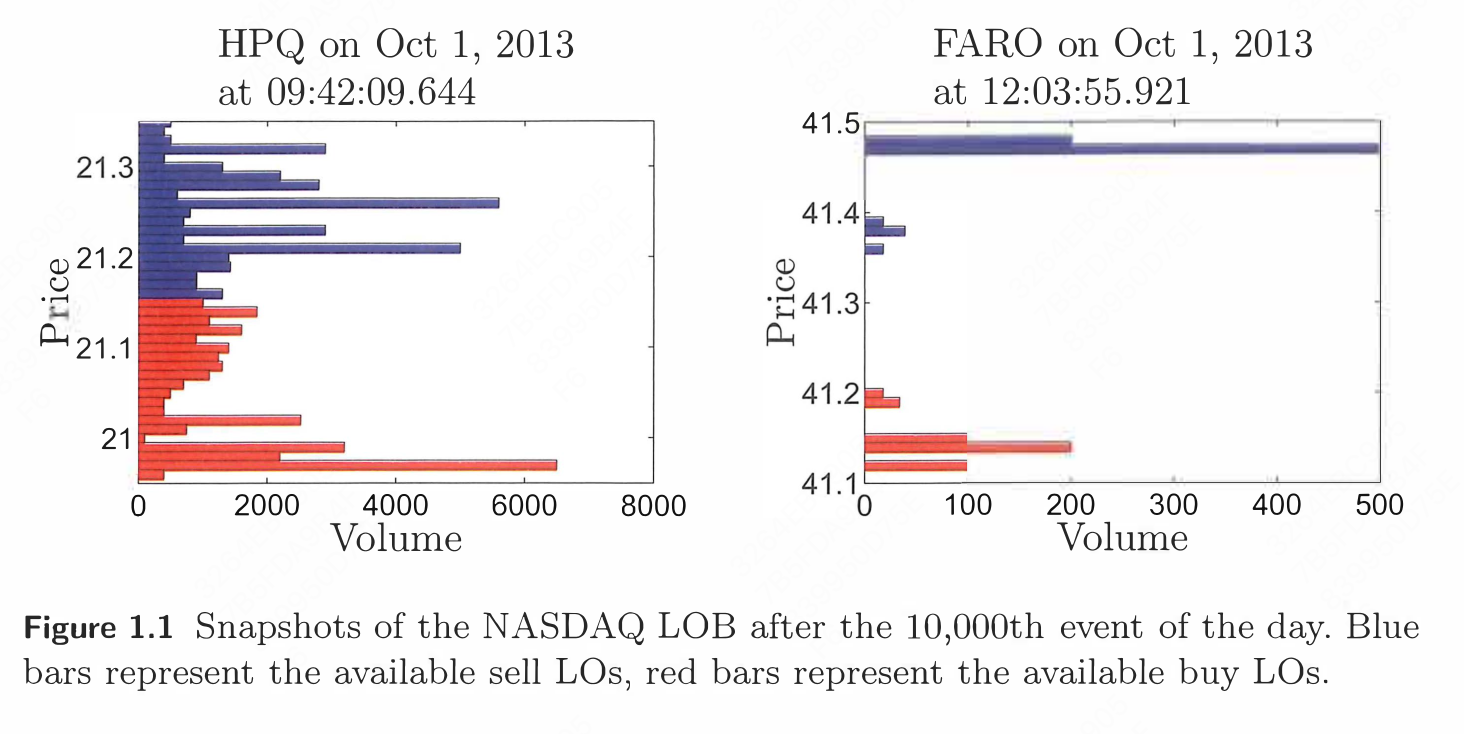
\includegraphics[width=.8\textwidth]{../images/Misc/15.png}
\label{f1.1}
\end{center}

Figure \ref{f1.1} shows a snapshot of the limit order book (LOB) on NASDAQ after the 10,000th event
of the day for two stocks, FARO and HPQ, on Oct 1, 2013. The two are quite different. The one in
the left panel corresponds to HPQ, a frequently traded and liquid asset. HPQ's LOB has LOs posted
at every tick out to (at least) 20 ticks away from the midprice. In the right panel, we have FARO's
LOB. FARO is a seldom traded, illiquid asset. This asset has thinly posted bids and offers and
irregular gaps in the LOB.
\subsubsection{Alternate Exchange Structures}
\label{sec:org2d23c4c}
The above approach is not the only possible way to organise an exchange. For example, one could use an
alternative matching algorithm, such as the \textbf{prorata rules} used in some money markets.

Beyond the legal definitions, we generically distinguish lit (open order book) from dark markets based
on whether limit book informa­ tion is publicly available or not.
\subsubsection{Colocation}
\label{sec:org17a0e8b}
Exchanges also control the amount and degree of granularity of the information you receive (e.g., you
can use the consolidated/public feed at a low cost or pay a relatively much larger cost for
direct/proprietary feeds from the exchanges). They also monetise the need for speed by renting out
computer/server space next to their matching engines, a process called \textbf{colocation}. Through colocation,
exchanges can provide uniform service to trading clients at competitive rates. Having the traders'
trading engines at a common location owned by the exchange simplifies the exchange's ability to
provide uniform service as it can control the hardware connecting each client to the trading engine,
the cable (so all have the same cable of the same length), and the network. This ensures that all
traders in colocation have the same fast access, and are not disadvantaged (at least in terms of
exchange-provided hardware).
\subsubsection{Extended Order Types}
\label{sec:org1bc5ee4}
\begin{itemize}
\item \textbf{Day Orders}: orders for trading during regular trading with options to extend to pre- or post-market sessions;
\item \textbf{Non-routable}: there are a number of orders that by choice or design avoid the default re-routing to
other exchanges, such as 'book only', 'post only', 'midpoint peg', \ldots{};
\item \textbf{Pegged, Hide-not-Slide}: orders that move with the midpoint or the national best price;
\item \textbf{Hidden}: orders that do not display their quantity;
\item \textbf{Iceberg}: orders that partially display their quantity (some have options so that the visible portion
will automatically be replenished when it is depleted by less than one round lot);
\item \textbf{Immediate-or-Cancel}: orders that execute as much as possible at the best price and the rest are
cancelled (such orders are not re-routed to another exchange nor do they walk the book);
\item \textbf{Fill-or-Kill}: orders sent to be executed at the best price in their entirety or not at all;
\item \textbf{Good-Till-Time}: orders with a fixed lifetime built into them so that they will be cancelled if not
executed by its expiration time;
\item \textbf{Discretionary}: orders display one price (the limit price) but may be executed at more aggressive
(hidden) prices;
\end{itemize}
\subsubsection{Exchange Fees}
\label{sec:orgc979b39}
\subsection{The Limit Order Book}
\label{sec:org5e7abf7}
\begin{center}
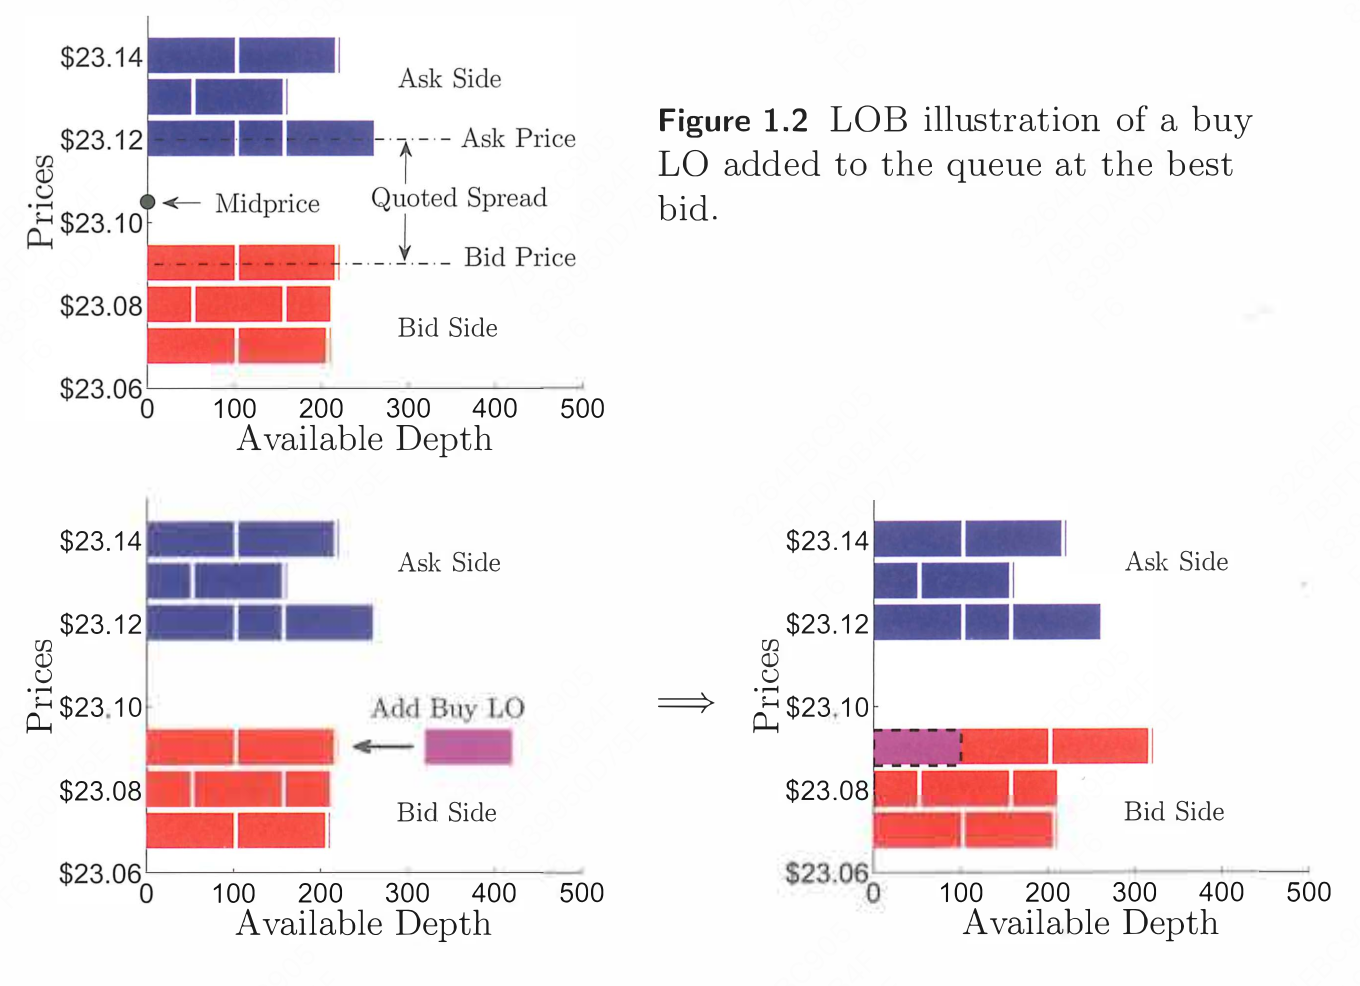
\includegraphics[width=.8\textwidth]{../images/Misc/16.png}
\label{f1.2}
\end{center}

\textbf{Addition of LO to LOB}. In Figure \ref{f1.2}, LOs are displayed as blocks of length equal to their
quantities. LOs are ordered in terms of time priority from right to left, so that when a new buy LO
comes in at \$23.09 (the purple block) it will be added to the line of blocks already at that price.
This new LO joins the queue at the point closest to the y-axis, becoming the third LO waiting to be
executed at \$23.09.

\begin{center}
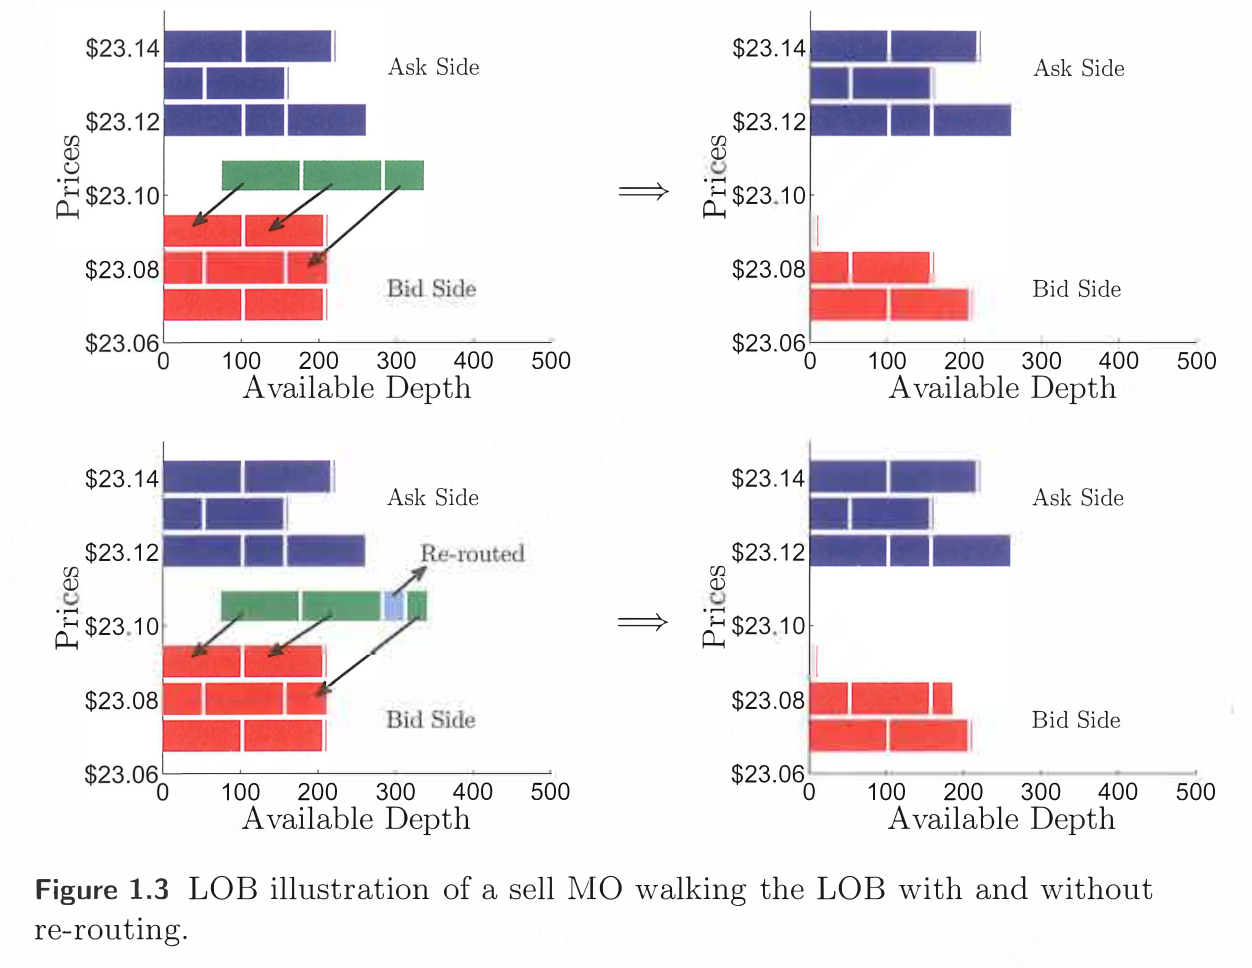
\includegraphics[width=.8\textwidth]{../images/Misc/17.png}
\label{f1.3}
\end{center}


\textbf{MO walks the LOB or is re-routed}. Suppose we are looking at the venue with the LOB depicted at the top
 of Figure \ref{f1.2}. Assume that this venue's best bid is the best buy quote that the market, across
 all venues, currently displays. A new MO (to sell) 250 shares enters this market as depicted by the
 sum of the green blocks in the top panel of Figure \ref{f1.3}. The matching engine goes through the
 LOB, matching existing (posted) LOs (to buy on the bid side) with the entering MO following the rules
 in the matching algorithm. In the LOB there are two LOs at the best bid \$23.09, represented by the
 two red blocks, both for 100 units, totalling 200 units. These 200 units are executed at the best
 bid.

What happens to the final 50 units depends on the order type and the market it is operating in.
In a standard market, the remaining 50 units will be executed against the LOs standing at \$23.08
ordered in terms of time-priority (the MO will 'walk the book'). This is captured by the top panels
in Figure \ref{f1.3}: the left panel shows that the MO coming in is split into three blocks, the first
two are matched with LOs at \$23.09 and the last with the LOs at \$23.08. After the MO is fully executed
the remaining LOB is shown in the top right panel of Figure \ref{f1.3}.

In the US, there are order protection rules to ensure MOs get the best possible execution, and which
(depending on the order type) may require the exchange to re-route the remaining 50 units to another
exchange that is also displaying a best bid price of \$23.09. In this case, as shown in the bottom left
panel of Figure \ref{f1.3}, part of the remaining 50 units (the light blue block) is re-routed to
another venue(s) with liquidity posted at \$23.09. Only once all liquidity at \$23.09 in all exchanges
is exhausted, can the remaining shares of the MO return and be executed in this venue against any LO
resting at (the worse price of) \$23.08. In this example, 25 units were re-routed to alternate
exchanges, and 25 units returned to this venue and walked the  book.

The MO could in principle be an Immediate-or-Cancel (IOC) order, which specifies that the remaining 50
shares that cannot be executed at the best bid should be cancelled entirely.

Because of these order protection rules (trade-through rules - there is no such rule in European
markets), you will very seldom observe in the US an MO walking the book straight away. Rather, you may
see a large MO being chopped up and executed sequentially in several markets in a very short span of
time. This also implies that as depth disappears (as during the Flash Crash of May 6th, 2010) an MO at
the end of a sequence of other orders may be executed against very poor prices, and, in the worst
circumstances it may be matched with \textbf{stub quotes} - LOs at prices so ridiculous that clearly indicate
they are not expected to be executed (such trades were observed during the Flash Crash in the
following assets: JKE, RSP, Excelon, Accenture, amongst others). Thus, the LOB serves to keep track of
LOs and apply the algorithm that matches incoming orders to existing LOs.

\index{tick}
The LOB is defined on a fixed discrete grid of prices (the price levels). The size of the step (the
difference between one price level and the next) is called the \textbf{tick}, and in the US the minimum tick
size is 1 cent for all stocks with a price above one dollar. In other markets several different tick
sizes coexist.

Figure \ref{f1.1} shows a sample plot of the limit order book (LOB) on NASDAQ after the 10,000th event
of the day for two stocks, FARO and HP Q, on Oct 1, 2013. In blue you find the sell LOs -traders
willing to wait to be able to sell at a high price. The best sell price, the ask, is \$21.16, while the
best buy price, the bid, is \$21.15. The difference between the ask and the bid price, the \textbf{quoted
spread} is
\begin{equation*}
\text{Quoted Spread}_t=P_t^a-P_t^b
\end{equation*}
where \(P_t^b\) and \(P_t^a\) are the best bid  and ask prices, which in this case, is one cent - the
minimum quoted spread. However, some times the bid is equal to the ask and the spread is zero. In that
case, the market becomes \textbf{locked}, but if this happens, it tends not to last long - although for some
very liquid assets it is becoming an increasingly more frequent event. Another common object used when
describing the LOB is the \textbf{midprice}. The midprice is the arithmetic average of the bid and the ask:
\begin{equation*}
\text{Midprice}_t=\frac{1}{2}(P_t^a+P^b_t)
\end{equation*}

As pointed out earlier, the two LOBs shown in Figure \ref{f1.1} are quite different. The one in the left
panel corresponds to HPQ, a frequently traded and liquid asset. HPQ's LOB has LOs posted at every tick
out to (at least) 20 ticks away  from the midprice and the spread is the minimum spread of 1 tick. In
the right panel, we have FARO's LOB. FARO is a seldom traded, illiquid asset. This asset has thinly
posted bids and offers and irregular gaps in the LOB. The spread is 20 ticks (20 cents) on a
(approximately) \$41 priced asset. The difference in liquidity between these assets is also noticeable
from the time at which the 10,000th event of the day takes place for these assets. For HPQ, the
10,000th event corresponds to a timestamp of about 9:42 a.m. (less than 15 minutes after the market
opened), while for FARO the 10,000th event did not occur until about 12:04 p.m. (more than two and a
half hours after market open). Also note that there are less than 100 units posted if we sum together
the depth at the best two price levels on the bid and ask for FARO, while for HPQ there are more than
1,000 shares offered in those first two levels of the LOB - HPQ thus has much greater depth. If one
takes into account that FARO trades at a price which is twice as high as that of HPQ, the depth in
terms of dollar value of shares posted at those prices is also much greater for HPQ.

\begin{center}
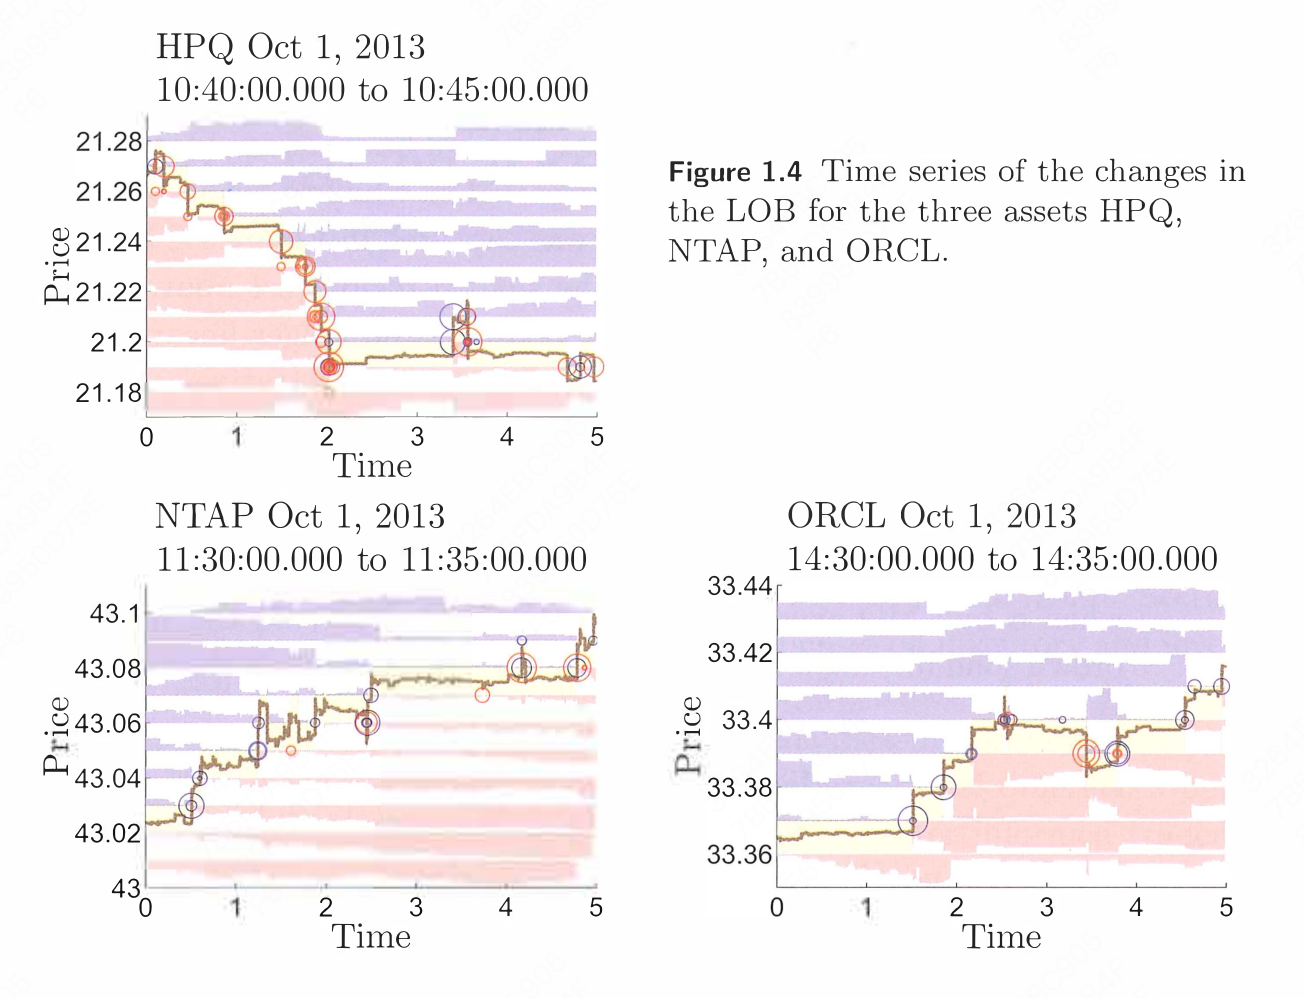
\includegraphics[width=.8\textwidth]{../images/Misc/18.png}
\label{f1.4}
\end{center}

In Figure \ref{f1.4}, we show how the LOB evolves through time for different stocks HPQ, NTAP and ORCL.
On the x-axis is time in minutes, and on the y-axis are prices in dollars. The static picture we saw
in Figure \ref{f1.1} is captured by the shaded blue and red regions - the blue regions on top represent
the ask side of the LOB, the posted sell volume, while the bid side is below in red, showing the
posted buy volume. The best prices, the bid and ask are identified by the edges of the intermediate
light shaded beige region, which identifies the bid-ask spread. Volume at each price level, which was
captured in Figure \ref{f1.1} by horizontal bars, is now illustrated by the size of the shaded region just
above/below each price level, although the height of these regions is no longer linear, but a
monotonic non-linear transformation that is visually more illustrative.

In addition, Figure \ref{f1.4} identifies when incoming orders were executed. The red/blue circles
indicate the time, price and size (indicated by the size of the circle) of an aggressive MO which is
executed against the LOs sitting in the LOB. When a sell MO executes against a buy LO, it is said to
\textbf{hit the bid}; analogously, when a buy MO executes against a sell LO, it is said the \textbf{lift the offer}. The
brown solid line depicts a variation of the asset known as the \textbf{microprice} defined as
\begin{equation*}
\text{Microprice}_t=\frac{V_t^b}{V_t^b+V_t^a}P_t^a+\frac{V_t^a}{V_t^b+V_t^a}P_t^b
\end{equation*}
where \(V_t^b\) and \(V_t^a\) are the volumes posted at the best bid and ask, and \(P_t^b\)
and |(P\textsubscript{t}\textsuperscript{a}) are the bid and ask prices.

The microprice is used as a more subtle proxy for the asset's transaction cost-free price, as it
measures the tendency that the price has to move either towards the bid or ask side as captured by
number of shares posted, and hence indicates the buy (sell) pressure in the market. If there are a lot
of buyers (sellers), then the microprice is pushed toward the best ask/bid price to reflect the
likelihood that prices are going to increase (decrease).
\section{A Primer on the Microstructure of Financial Markets}
\label{sec:org80d317a}
\subsection{Market Making}
\label{sec:orgc6608d3}
\subsubsection{Grossman-Miller Market Making Model}
\label{sec:org0b7c520}
The first issue faced by an MM when providing liquidity is that by accepting one side of a trade (say
buying from someone who wants to sell), the MM will hold an asset for an uncertain period of time, the
time it takes for another person to come to the market with a matching demand for liquidity (wanting
to buy the asset the MM bought in the previous trade). During that time, the MM is exposed to the risk
that the price moves against her (in our example, as she bought the asset, she is exposed to a price
decline and hence having to sell the asset at a loss in the next trade).

Grossman \& Miller (1988) provide a model that captures this problem and describes how MMs obtain a
liquidity premium from liquidity traders that exactly compensates MMs for the price risk of holding an
inventory of the asset until they can unload it later to another liquidity trader.

Let us consider a simplified version of their model, with a finite number, \(n\), of identical MMs for
some given asset and three dates \(t\in\{1,2,3\}\). To simplify the situation, there is no uncertainty
about the arrival of matching orders: if at date \(t=1\) a liquidity trader, denoted by LT1, comes to
the market to sell \(i\) units of the asset, there will be (for sure) another liquidity trader (LT2)
who will arrive at the market to purchase \(i\) units (or more generally, to trade \(-i\) units, so
that LT1's trade (of i units) could be negative or positive (LT1 could be buying or selling). However,
LT2 does not arrive to the market until \(t=2\). Let all agents start with an initial cash amount
equal to \(W_0\) , MMs hold no assets, LT1 holds \(i\) units and LT2 \(-i\) units.

There are no trading costs or direct costs for holding inventory. The focus is on price changes: the
asset will have a cash value at \(t=3\) of \(S_3=\mu+\epsilon_2+\epsilon_3\), where \(\mu\) is
constant, \(\epsilon_2\) and \(\epsilon_3\) are independent, normally distributed random variables
with mean zero and variance \(\sigma^2\) . These will be publicly announced between dates \(t-1\) and
\(t\), that is \(\epsilon_3\) is announced between \(t=2\) and \(t=3\), and \(\epsilon_2\)is announced
between \(t=1\) and \(t=2\). Hence, the realised cash value of the asset can increase or decrease
(ignore the fact that there are realisations of \(\epsilon_2\) and \(\epsilon_3\) that could make the
asset value negative - the model serves to illustrate a point). Because the shocks to the value of the
asset are on average zero a risk-neutral trader has no cost at all from holding the asset. The model
becomes interesting if we assume that all traders, MMs and liquidity traders, are risk-averse. To be
more specific, suppose they have the following expected utility for the future random cash value of
the asset (\(X_3\)): \(\E[U(X_3)]\) where \(U(X)=-\exp(-\gamma X)\), and where \(\gamma>0\) is a
parameter capturing the utility penalty for taking risks

Solving the model backwards we obtain a description of trading behaviour and prices. At \(t=3\) the
cash value of the asset is realised, \(S_3=\mu+\epsilon_2+\epsilon_3\). At \(t=2\), the \(n\) MMs and
LT1 come into the period with asset holdings \(q_1^{MM}\) and \(q_1^{LT1}\) respectively. LT2 comes in
with \(-i\) and they all exit with asset holdings \(q_2^j\), where \(j\in\{MM,LT1,LT2\}\). Note that
if, for example, \(q_t^j=2\) this denotes the that agent \(j\) is holding 2 units when exiting date
\(t\), so that the agent will be long (that is, has an iventory of) two units.

Given the problem as described so far, at \(t=2\) agent \(j\) chooses \(q_2^j\) to maximise his
expected utility knowing the realisation of \(\epsilon_2\) that was made public before \(t=2\):
\begin{equation*}
\max_{q_2^j}\E\left[ U(X_3^j)|\epsilon_2 \right]
\end{equation*}
subject to
\begin{gather*}
X_3^j=X_2^j+q_2^jS_3\\
X_2^j+q_2^jS_2=X_1^j+q_1^jS_2
\end{gather*}
These two contraints capture:
\begin{enumerate}
\item the fact that the cash value of the agent's assets at \(t=3\), \(X_3\), is equal to the agent's
cash holdings at \(t=3\), which is equal to \(X_2\) plus the cash value of the agent's asset
inventory \(q_2^j\)
\item the fact that the cash value of the agent's assets when exiting date \(t=2\) was equal to the cash
value of the agent's assets when entering date \(t=2\)
\end{enumerate}

Given the normality assumption and the properties of the expected utility function it is
straightforward to show that
\begin{align*}
\E\left[ U(X_3^j)|\epsilon_2 \right]&=-\exp\left\{
-\gamma\left( X_2^j+q_2^j\E[S_3|\epsilon_2] \right)+\frac{1}{2}\gamma^2\left( q_2^j \right)^2\sigma^2 \right\}
\end{align*}
\wu{
Since \(\epsilon_2\) and \(\epsilon_3\) are independent, \(\epsilon_3|\epsilon_2\sim N(0,\sigma^2)\)
Therefore \(S|\epsilon_2=y=\mu+y+\epsilon_3|\epsilon_2=y\sim N(\mu+y,\sigma^2)\)
Then \(S|\epsilon_2\sim N(\mu+\epsilon_3,\sigma^2)\)
Let \(\mu=\E[S_3|\epsilon_2]\). Then \(S|\epsilon\sim N(\mu,\sigma^2)\).

Assume \(X\sim N(\mu,\sigma^2)\). The \textbf{Moment generating function} (\textbf{MGF}) is
\begin{equation*}
M_X(t)=\E[e^{tX}]=\int_{-\infty}^{\infty}e^{tx}\cdot\frac{1}{\sigma\sqrt{2\pi}}e^{\frac{(x-\mu)^2}{2\sigma^2}}dx
\end{equation*}
As
\begin{align*}
tx-\frac{(x-\mu)^2}{2\sigma^2}&=\frac{2\sigma^2tx-(x^2-2\mu x+\mu^2)}{2\sigma^2}\\
&=-\frac{x^2-2\mu x-2\sigma^2tx+\mu^2}{2\sigma^2}\\
&=-\frac{x^2-2x(\mu+\sigma^2t)+\mu^2}{2\sigma^2}\\
&=-\frac{(x-(\mu+\sigma^2t))^2-2\mu\sigma^2t-\sigma^4t^2}{2\sigma^2}
\end{align*}
We have
\begin{equation*}
M_x(t)=e^{ut+\frac{\sigma^2t^2}{2}}\int_{-\infty}^\infty\frac{1}{\sigma\sqrt{2\pi}}e^{-\frac{x-(\mu+\sigma^2t)^2}{2\sigma^2}}
\end{equation*}
The integral is the PDF (probability density function) of a \(N(\mu+\sigma^2t,\sigma^2)\)
distribution, which integrates to 1. Thus
\begin{equation*}
M_X(t)=\exp\left\{\mu t+\frac{\sigma^2t^2}{2}\right\}
\end{equation*}

Now
\begin{align*}
\E[U(X_3^j)\mid\epsilon_2]&=\E[-\exp\left\{ -\gamma_(X_2^j+q_2^jS_3) \right\}\mid\epsilon_2]\\
&=-\exp\{-\gamma X_2^j\}\cdot\E[\exp\{-\gamma q_2^jS_3\}\mid\epsilon_2]\\
&=-\exp\{-\gamma X_2^j\}\cdot\exp\left\{ -\gamma q_2^j\mu+\frac{1}{2}\gamma^2(q_2^j)^2\sigma^2 \right\}
\end{align*}
where \(\mu=\E[S_3\mid\epsilon_2]\)
}

Thus, the problem is concave and the solution is characterized by
\begin{equation*}
q_2^{j,*}=\frac{\E[S_3\mid\epsilon_3]-S_2}{\gamma\sigma^2}
\end{equation*}
for all agents: the \(n\) MMs, LT1, and LT2

As at date \(t=2\) demand and supply for the asset have to be equal to each other, we can solve for
the equilibrium price \(S_2\):
\begin{equation}
\label{e2.1}
nq_1^{MM}+q_1^{LT_1}+q_1^{LT2}=nq_2^{MM}+q_2^{LT1}+q_2^{LT2}
\end{equation}
As we have established above, all \(q_2^j\) are equal, so that the right-hand side of the above
equation is equal to
\begin{equation}
\label{e2.2}
nq_2^{MM}+q_2^{LT1}+q_2^{LT2}=(n+2)\frac{\E[S_3\mid\epsilon_2]-S_2}{\gamma\sigma^2}
\end{equation}
We also know that at date 1 the total quantity of the asset available was equal to the quantity of
assets LT1 brought to the market, so that LHS of \eqref{e2.1} is
\begin{equation*}
nq_1^{MM}+q_1^{LT1}+q_1^{LT2}=i-i=0
\end{equation*}
Hence, we obtain that in equilibrium, at date \(t=2\),
\(S_2=\E[S_3]=\mu+\epsilon_2+\E[\epsilon_3]=\mu+\epsilon_2\), and therefore \(q_2^j=0\).

\begin{center}
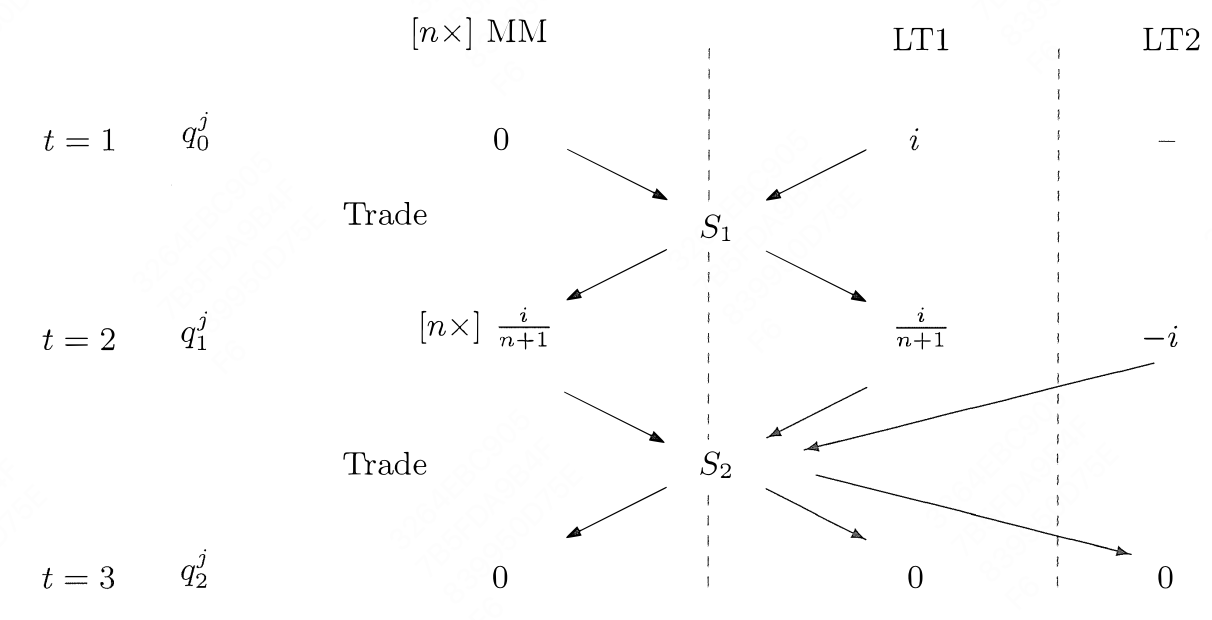
\includegraphics[width=.8\textwidth]{../images/Misc/19.png}
\captionof{figure}{\label{f2.1}Trading and price setting in the Grossman-Miller model}
\end{center}


This makes sense, as at \(t=2\) there are no asset imbalances, the price of the asset reflects its
'fundamental value' and no one will want to hold a non-zero amount of the risky asset. This analysis
is captured in the bottom half of Figure \ref{f2.1}, where we see the asset holdings of the three types
of participants as they enter \(t=2\), \(q_1^j\), \(j\in\{MM,LT1,LT2\}\), and how after trading at a
price equal to \(S_2\) they end up with holdings, \(q_2^j\), equal to zero

Consider now what happens at date \(t=1\). Participating agents (the \(n\) MMs and LT1) anticipate
that whatever they do, the future market price will be efficient and they will end up exiting date
\(t=2\) with no inventories, so that \(X_2=X_3\). Thus, their portfolio decision is given by
\begin{equation*}
\max_q\E\left[ U(X_2^j) \right]
\end{equation*}
subject to
\begin{gather*}
X_2^j=X_1^j+q_1^jS_1\\
X_1^j+q_1^jS_1=X_0^j+q_0^jS_1
\end{gather*}
\end{document}
